\documentclass[a4paper,11pt]{report}
\usepackage[showexo=true,showcorr=false]{../packages/coursclasse}
%Commenter ou enlever le commentaire sur la ligne suivante pour montrer le niveau
\toggletrue{montrerNiveaux}
%permet de gérer l'espacement entre les items des env enumerate et enumitem
\usepackage{enumitem}
\setlist[enumerate]{align=left,leftmargin=1cm,itemsep=10pt,parsep=0pt,topsep=0pt,rightmargin=0.5cm}
\setlist[itemize]{align=left,labelsep=1em,leftmargin=*,itemsep=0pt,parsep=0pt,topsep=0pt,rightmargin=0cm}
%permet de gerer l'espacement entre les colonnes de multicols
\setlength\columnsep{35pt}

\begin{document}

%%%%%%%%%%%%%%%%% À MODIFIER POUR CHAQUE SERIE %%%%%%%%%%%%%%%%%%%%%%%%%%%%%
\newcommand{\chapterName}{Grandeurs et mesures}
\newcommand{\serieName}{Volume et aire totale de solides}


%%%%%%%%%%%%%%%%%% PREMIERE PAGE NE PAS MODIFER %%%%%%%%%%%%%%%%%%%%%%%%
% le chapitre en cours, ne pas changer au cours d'une série
\chapter*{\chapterName}
\thispagestyle{empty}

%%%%% LISTE AIDE MEMOIRE %%%%%%
\begin{amL}{\serieName}{
\item Volume d'un solide (généralités) (page 169)
\item Volume des solides usuels (page 170)
\item Calculer le volume d'un solide (page 172)
\item Polyèdre (page 144)
\item Prisme droit (page 145)
\item Parallélépipède rectangle ou pavé droit (page 146)
}\end{amL}

%%%%%%%%%%%%%%% DEBUT DE LA SERIE NE PAS MODIFIER %%%%%%%%%%%%%%%%%%%%%%%%%%%%%
\section*{\serieName}
\setcounter{page}{1}
\thispagestyle{firstPage}



%%%%%%%%%%% LES EXERCICES %%%%%%%%%%%%%%%%%%%%%%%%%%%%%%%%%%%%






\begin{resolu}{Calculer le volume d'un solide en cubes-unité}{
\begin{minipage}[t]{0.6\textwidth}{
\vspace{0pt}
\begin{tasks}(1)[after-item-skip = 0.3em]
    \task Calcule le volume du solide ci-contre en utilisant le cube comme unité. Remarque : les cubes cachés n'ont pas été dessinés. 
\end{tasks}
}
\end{minipage}
\begin{minipage}[t]{0.4\textwidth}{
\vspace{0pt}
\begin{center}
\begin{tikzpicture}[scale=0.7]
    %\drawbox{x}{z}{y}{}
    \drawbox{1}{3}{3}{}
    \drawbox{2}{3}{3}{}
    \drawbox{3}{3}{1}{}
    \drawbox{3}{3}{2}{}
    \drawbox{1}{2}{1}{}
    \drawbox{1}{2}{2}{}
    \drawbox{2}{2}{1}{}
    \drawbox{2}{2}{2}{}
    \drawbox{2}{2}{3}{}
    \drawbox{3}{2}{1}{}
    \drawbox{3}{2}{2}{}
    \drawbox{3}{2}{3}{}
    \drawbox{2}{1}{1}{}
    \drawbox{3}{1}{1}{}
    \drawbox{3}{1}{2}{}    
\end{tikzpicture}
\end{center}
}
\end{minipage}

\begin{tasks}[after-item-skip = 0.3em] 
	\task[]     \uline{En prenant en compte les cubes cachés, je comptabilise 19 cubes au total (8 au premier étage, 7 au deuxième étage et 4 au dernier étage). Le volume du solide est de 19 cubes-unité.}
	\task[b)] Quel serait son volume si le cube-unité a un volume de $\tunit{1}{\centi m^3}$ ? 

    \uline{Si un cube a un volume de $\tunit{1}{\centi m^3}$, alors le volume du solide correspond à $\tunit{19}{\centi m^3}$}
    
    \task[c)] Quel serait son volume si le cube-unité a un volume de $\tunit{3}{\centi m^3}$ ? 
    
    \uline{Si un cube a un volume de $\tunit{3}{\centi m^3}$, alors le volume du solide correspond à $19\cdot3=\tunit{57}{\centi m^3}$}
\end{tasks}
}{1}    
\end{resolu}

\begin{exo}{
		\begin{minipage}[t]{0.6\textwidth}{
		\vspace{0pt}	
\begin{tasks}(1)[after-item-skip = 0.3em]
    \task Calcule le volume du solide ci-contre en utilisant le cube comme unité. Remarque : les cubes cachés n'ont pas été dessinés. 
\end{tasks}
		}
		\end{minipage}
		\begin{minipage}[t]{0.4\textwidth}{
		\vspace{0pt}
\begin{center}
\begin{tikzpicture}[scale=0.7]
    %\drawbox{x}{z}{y}{}
    \drawbox{1}{3}{2}{}
    \drawbox{2}{3}{2}{}
    \drawbox{1}{3}{3}{}
    \drawbox{2}{3}{3}{}
    \drawbox{3}{3}{1}{}
    \drawbox{3}{3}{2}{}
    \drawbox{3}{3}{2}{}
    
    \drawbox{1}{2}{1}{}
    \drawbox{2}{2}{1}{}
    \drawbox{1}{2}{2}{}
    \drawbox{2}{2}{2}{}
    
    \drawbox{1}{1}{1}{}
    \drawbox{2}{1}{1}{}
    \drawbox{1}{1}{2}{}
    \drawbox{2}{1}{2}{}
    \drawbox{1}{1}{3}{}
    
\end{tikzpicture}
\end{center}

		}
		\end{minipage}
		\begin{tasks}[after-item-skip = 0.3em]
			\task[b)] Quel serait son volume si le cube-unité a un volume de $\tunit{1}{\centi m^3}$ ?
			\task[c)] Quel serait son volume si le cube-unité a un volume de $\tunit{3}{\centi m^3}$ ?
\end{tasks}
}{1}
\end{exo}

\begin{exo}{
		\begin{minipage}[t]{0.6\textwidth}{
		\vspace{0pt}
		\begin{tasks}(1)[after-item-skip = 0.3em]
    \task Calcule le volume du solide ci-contre en utilisant le cube comme unité. Remarque : les cubes cachés n'ont pas été dessinés. 
\end{tasks}
		}
		\end{minipage}
		\begin{minipage}[t]{0.4\textwidth}{
		\vspace{0pt}
\begin{center}
\begin{tikzpicture}[scale=0.7]
    %\drawbox{x}{z}{y}{}
    \drawbox{1}{3}{4}{}
    \drawbox{2}{3}{2}{}
    \drawbox{2}{3}{3}{}
    \drawbox{3}{3}{1}{}
    \drawbox{3}{3}{2}{}
    \drawbox{3}{3}{3}{}
    \drawbox{1}{2}{2}{}
    \drawbox{1}{2}{3}{}
    \drawbox{2}{2}{1}{}
    \drawbox{3}{2}{1}{}
    \drawbox{1}{1}{1}{}
    \drawbox{1}{1}{2}{}
    \drawbox{2}{1}{1}{}
    \drawbox{3}{1}{1}{}
    \drawbox{3}{1}{2}{}
    %\drawbox{1}{1}{3}{}
\end{tikzpicture}
\end{center}
		}
		\end{minipage}
		\begin{tasks}[after-item-skip = 0.3em]
			\task[b)] Quel serait  son volume si le cube-unité a un volume de $\tunit{1}{\deci m^3}$ ? 
			\task[c)] Quel serait  son volume si le cube-unité a un volume de $\tunit{5}{\deci m^3}$ ? 
\end{tasks}
}{1}
\end{exo}

\begin{exo}{
\begin{minipage}[t]{0.6\textwidth}{
\vspace{0pt}
\begin{tasks}(1)[after-item-skip = 0.3em]
    \task Calcule le volume du solide ci-contre en utilisant le cube comme unité. Remarque : les cubes cachés n'ont pas été dessinés. 
\end{tasks}
}
\end{minipage}
\begin{minipage}[t]{0.4\textwidth}{
\vspace{0pt}
\begin{center}
\begin{tikzpicture}[scale=0.7]
    %\drawbox{x}{z}{y}{}
    \drawbox{1}{3}{1}{}
    \drawbox{1}{3}{2}{}
    \drawbox{1}{3}{3}{}
    \drawbox{1}{3}{4}{}
    \drawbox{2}{3}{3}{}
    \drawbox{2}{3}{4}{}
    \drawbox{3}{3}{1}{}
    \drawbox{3}{3}{2}{}
    \drawbox{1}{2}{1}{}
    \drawbox{2}{2}{1}{}
    \drawbox{3}{2}{1}{}
    \drawbox{3}{2}{2}{}
    \drawbox{3}{2}{3}{}
    \drawbox{3}{2}{4}{}
    \drawbox{1}{1}{1}{}
    \drawbox{1}{1}{2}{}
    \drawbox{2}{1}{1}{}
    \drawbox{3}{1}{1}{}
    \drawbox{3}{1}{2}{}
    \drawbox{3}{1}{3}{}
\end{tikzpicture}
\end{center}
}
\end{minipage}
\begin{tasks}[after-item-skip = 0.3em]
	\task[b)] Quel serait  son volume si le cube-unité a un volume de $\tunit{1}{\deca m^3}$ ? 
	\task[c)] Quel serait  son volume si le cube-unité a un volume de $\tunit{20}{\deca m^3}$ ? 
\end{tasks}
}{1}
\end{exo}

\begin{exo}{
		\begin{minipage}[t]{0.6\textwidth}{
		\vspace{0pt}
	\begin{tasks}(1)[after-item-skip = 0.3em]
    \task Calcule le volume du solide ci-contre en utilisant le cube comme unité. Remarque : les cubes cachés n'ont pas été dessinés. 	
\end{tasks}
		}
		\end{minipage}
		\begin{minipage}[t]{0.4\textwidth}{
		\vspace{0pt}
\begin{center}
\begin{tikzpicture}[scale=0.7]
    %\drawbox{x}{z}{y}{}
    \drawbox{1}{3}{3}{}
    \drawbox{2}{3}{2}{}
    \drawbox{3}{3}{1}{}
    \drawbox{3}{3}{2}{}
    \drawbox{3}{3}{3}{}
    \drawbox{1}{2}{2}{}
    \drawbox{2}{2}{1}{}
    \drawbox{3}{2}{1}{}
    \drawbox{3}{2}{2}{}
    \drawbox{1}{1}{1}{}
    \drawbox{1}{1}{2}{}
    \drawbox{1}{1}{3}{}
    \drawbox{2}{1}{1}{}
\end{tikzpicture}
\end{center}
		}
		\end{minipage}


		\begin{tasks}[after-item-skip = 0.3em]
			\task[b)] Quel serait  son volume si le cube-unité a un volume de $\tunit{1}{\hecto m^3}$ ? 
			\task[c)] Quel serait  son volume si le cube-unité a un volume de $\tunit{1,5}{\hecto m^3}$ ? 
\end{tasks}
}{1}
\end{exo}


\begin{exo}{
		\begin{minipage}[t]{0.6\textwidth}{
		\vspace{0pt}
		Cet escalier est fait de cubes empilés. Chaque cube a un volume de $27\un{cm^3}$. Quel est le volume de l'escalier ?
		}
		\end{minipage}
		\begin{minipage}[t]{0.4\textwidth}{
		\vspace{0pt}
\begin{center}
\begin{tikzpicture}[scale=0.7]
    %\drawbox{x}{z}{y}{}
    \drawbox{1}{2}{3}{}
    \drawbox{2}{2}{2}{}
    \drawbox{3}{2}{1}{}
    
    \drawbox{1}{1}{1}{}
    \drawbox{1}{1}{2}{}
    \drawbox{1}{1}{3}{}

    \drawbox{2}{1}{1}{}
    \drawbox{2}{1}{2}{}

    \drawbox{3}{1}{1}{}
\end{tikzpicture}
\end{center}		}
		\end{minipage}
}{1}
\end{exo}



\begin{exo}{
Calcule le volume des prismes droits décrits ci-dessous.
\begin{tasks}[after-item-skip = 0.2em]
    \task Un parallélépipède rectangle dont une des bases est un rectangle de $\tunit{50}{\centi m^2}$ d'aire et dont la hauteur mesure $\tunit{2}{\centi m}$.
    \task Un prisme droit dont la base est un triangle de $\tunit{40}{m^2}$ d'aire et dont la hauteur mesure $\tunit{6}{m}$.
    \task Un parallélépipède rectangle dont une des bases est un carré de $\tunit{2,5}{\hecto m^2}$ d'aire et dont la hauteur mesure $\tunit{4}{\hecto m}$.
    \task Un prisme droit dont la base est un hexagone de $\tunit{0,8}{\deca m^2}$ d'aire et dont la hauteur mesure $\tunit{9}{\deca m}$.
    \task Un prisme droit dont la base est un rectangle de $\tunit{0,5}{m^2}$ d'aire et dont la hauteur mesure $\tunit{5}{\deci m}$.
    \task Un prisme dont une des bases est un rectangle de $\tunit{1,2}{\kilo m^2}$ d'aire et dont la hauteur mesure $\tunit{0,04}{\deca m}$.
\end{tasks}
\vspace{-0.3cm}
}{1}
\end{exo}


%volume cube, pavé droit (+ conversion d'unité)
\begin{exo}{
Calcule le volume d'un cube dont l'arête vaut :
\begin{tasks}[after-item-skip = 0.3em](3)
    \task $\tunit{3}{\centi m}$
    \task $\tunit{5}{\deca m}$
    \task $\tunit{10}{\hecto m}$
    \task $\tunit{40}{\milli m}$
    \task $\tunit{500}{\deci m}$
    \task $\tunit{0,1}{\kilo m}$
    \task $\tunit{0,9}{m}$
    \task $\tunit{0,03}{\deca m}$
    \task $\tunit{1,5}{\centi m}$
\end{tasks}
}{1}
\end{exo}

\begin{exo}{
Calcule le volume d'un parallélépipède rectangle dont les dimensions sont :
\begin{tasks}(2)[after-item-skip = 0.3em]
    \task  $\tunit{5}{\deci m}$, $\tunit{2}{\deci m}$ et $\tunit{3}{\deci m}$
    \task  $\tunit{7}{m}$, $\tunit{8}{m}$ et $\tunit{2}{m}$
    \task  $\tunit{0,5}{\hecto m}$, $\tunit{3}{\hecto m}$ et $\tunit{5}{\hecto m}$
    \task  $\tunit{9}{\deca m}$, $\tunit{10}{\deca m}$ et $\tunit{0,25}{\deca m}$
    \task  $\tunit{0,3}{\deca m}$, $\tunit{6}{m}$ et $\tunit{90}{\deci m}$
    \task  $\tunit{0,4}{m}$, $\tunit{5}{\deci m}$ et $\tunit{10}{\centi m}$
    \task  $\tunit{0,15}{\kilo m}$, $\tunit{6}{\deca m}$ et $\tunit{2,5}{\hecto m}$
    \task  $\tunit{0,2}{\deci m}$, $\tunit{4}{\milli m}$ et $\tunit{1,8}{\centi m}$
\end{tasks}
\vspace{-0.3cm}
}{1}
\end{exo}

\begin{exo}{
Calcule le volume des pavés droits représentés ci-dessous. Toutes les mesures sont exprimées en $\tunit{}{\centi m}$.

\begin{tasks}[after-item-skip = 0em](2)
    \task ~\\ 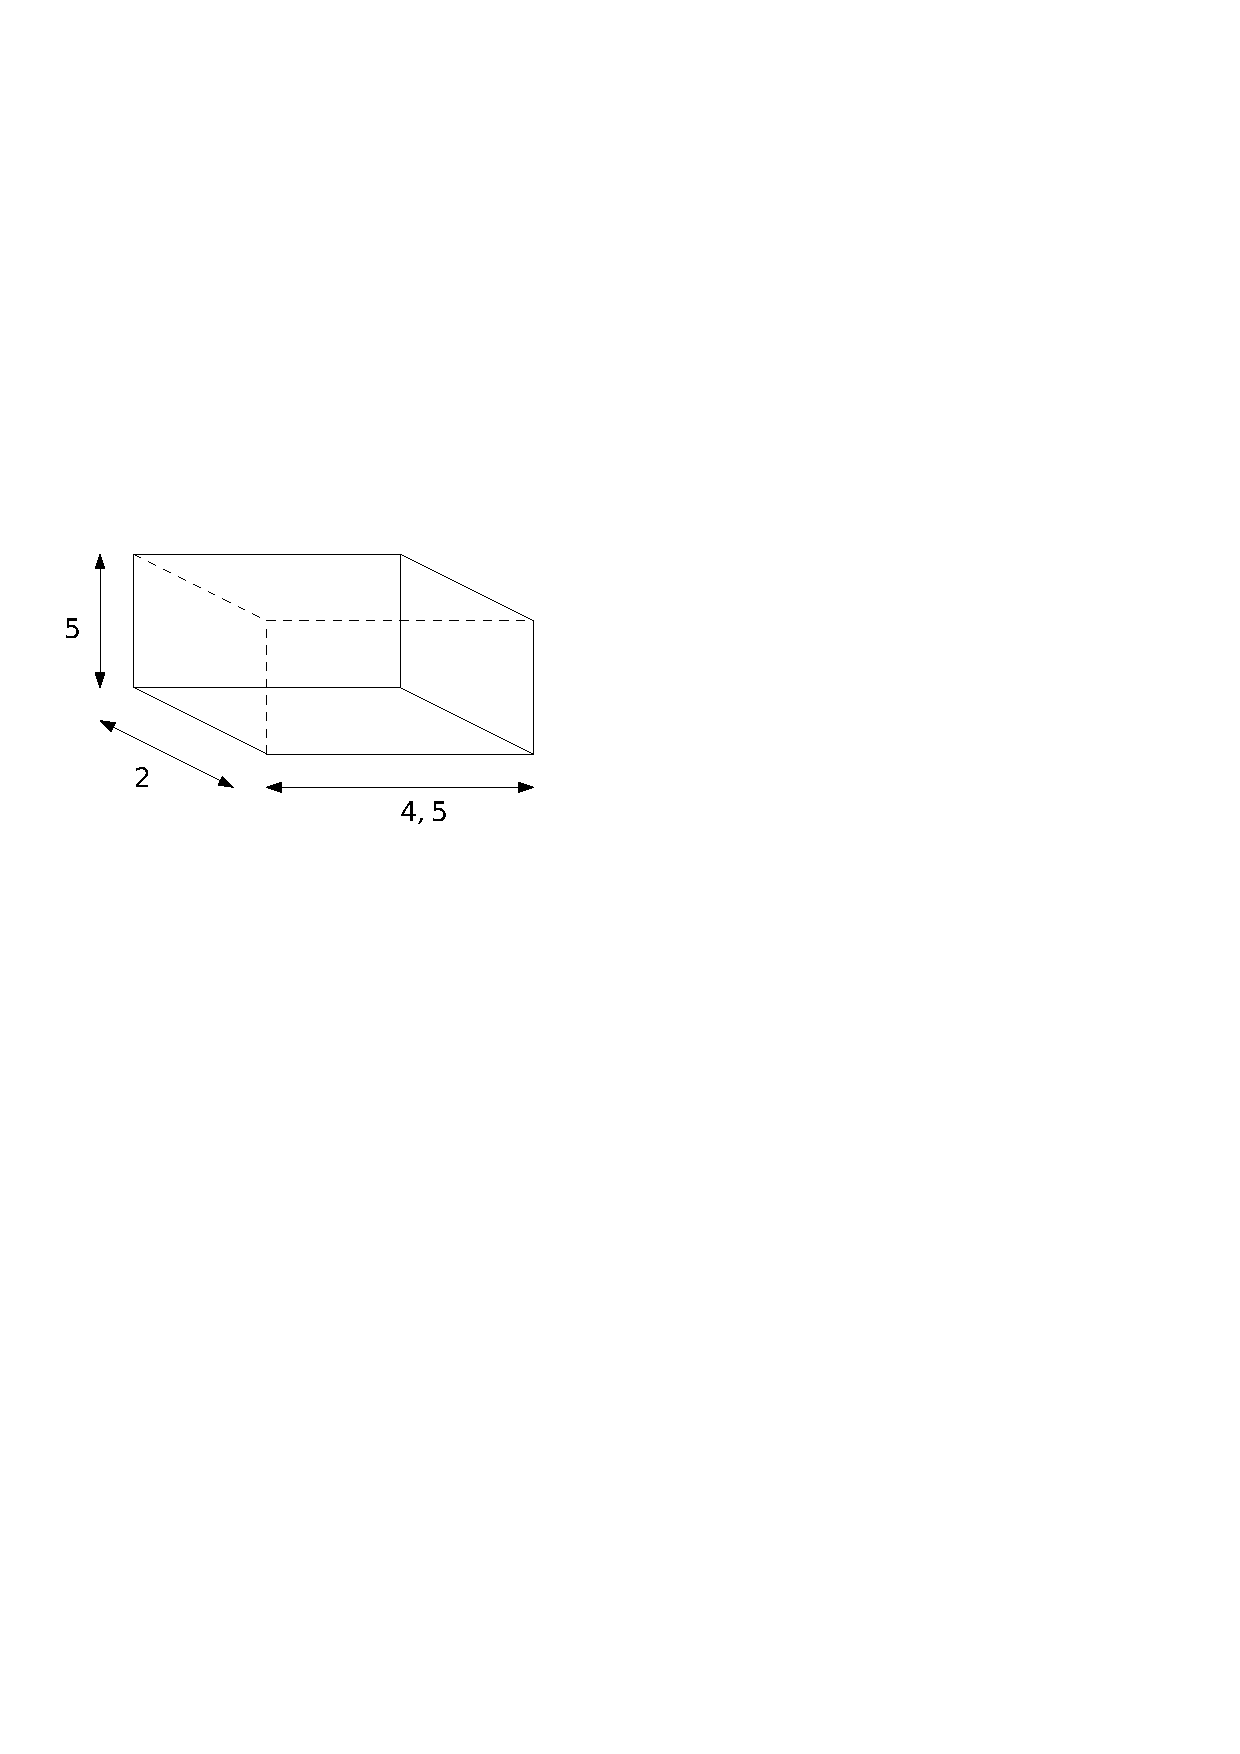
\includegraphics[scale=0.5]{media/gm-02/pave1.pdf}
    \task ~\\ 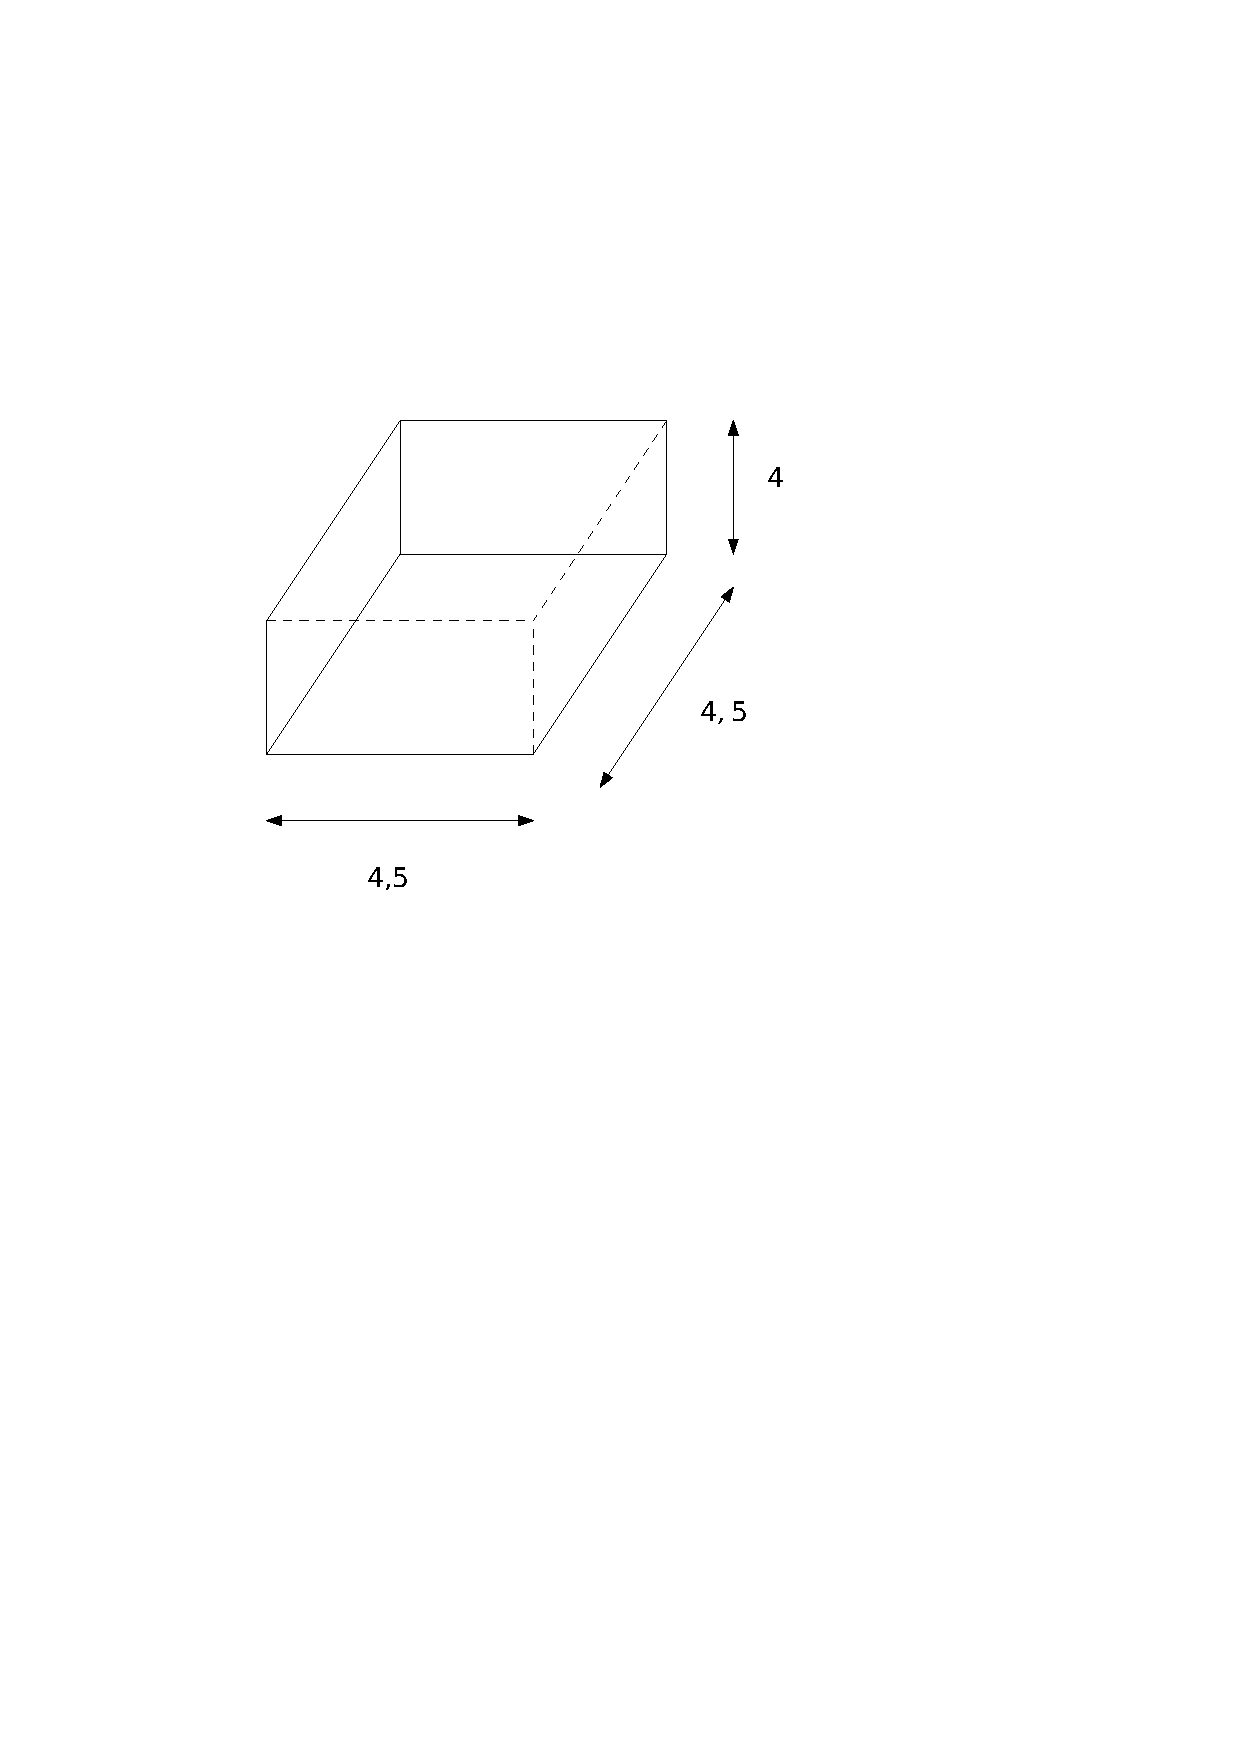
\includegraphics[scale=0.5]{media/gm-02/pave2.pdf}
    \task ~\\ 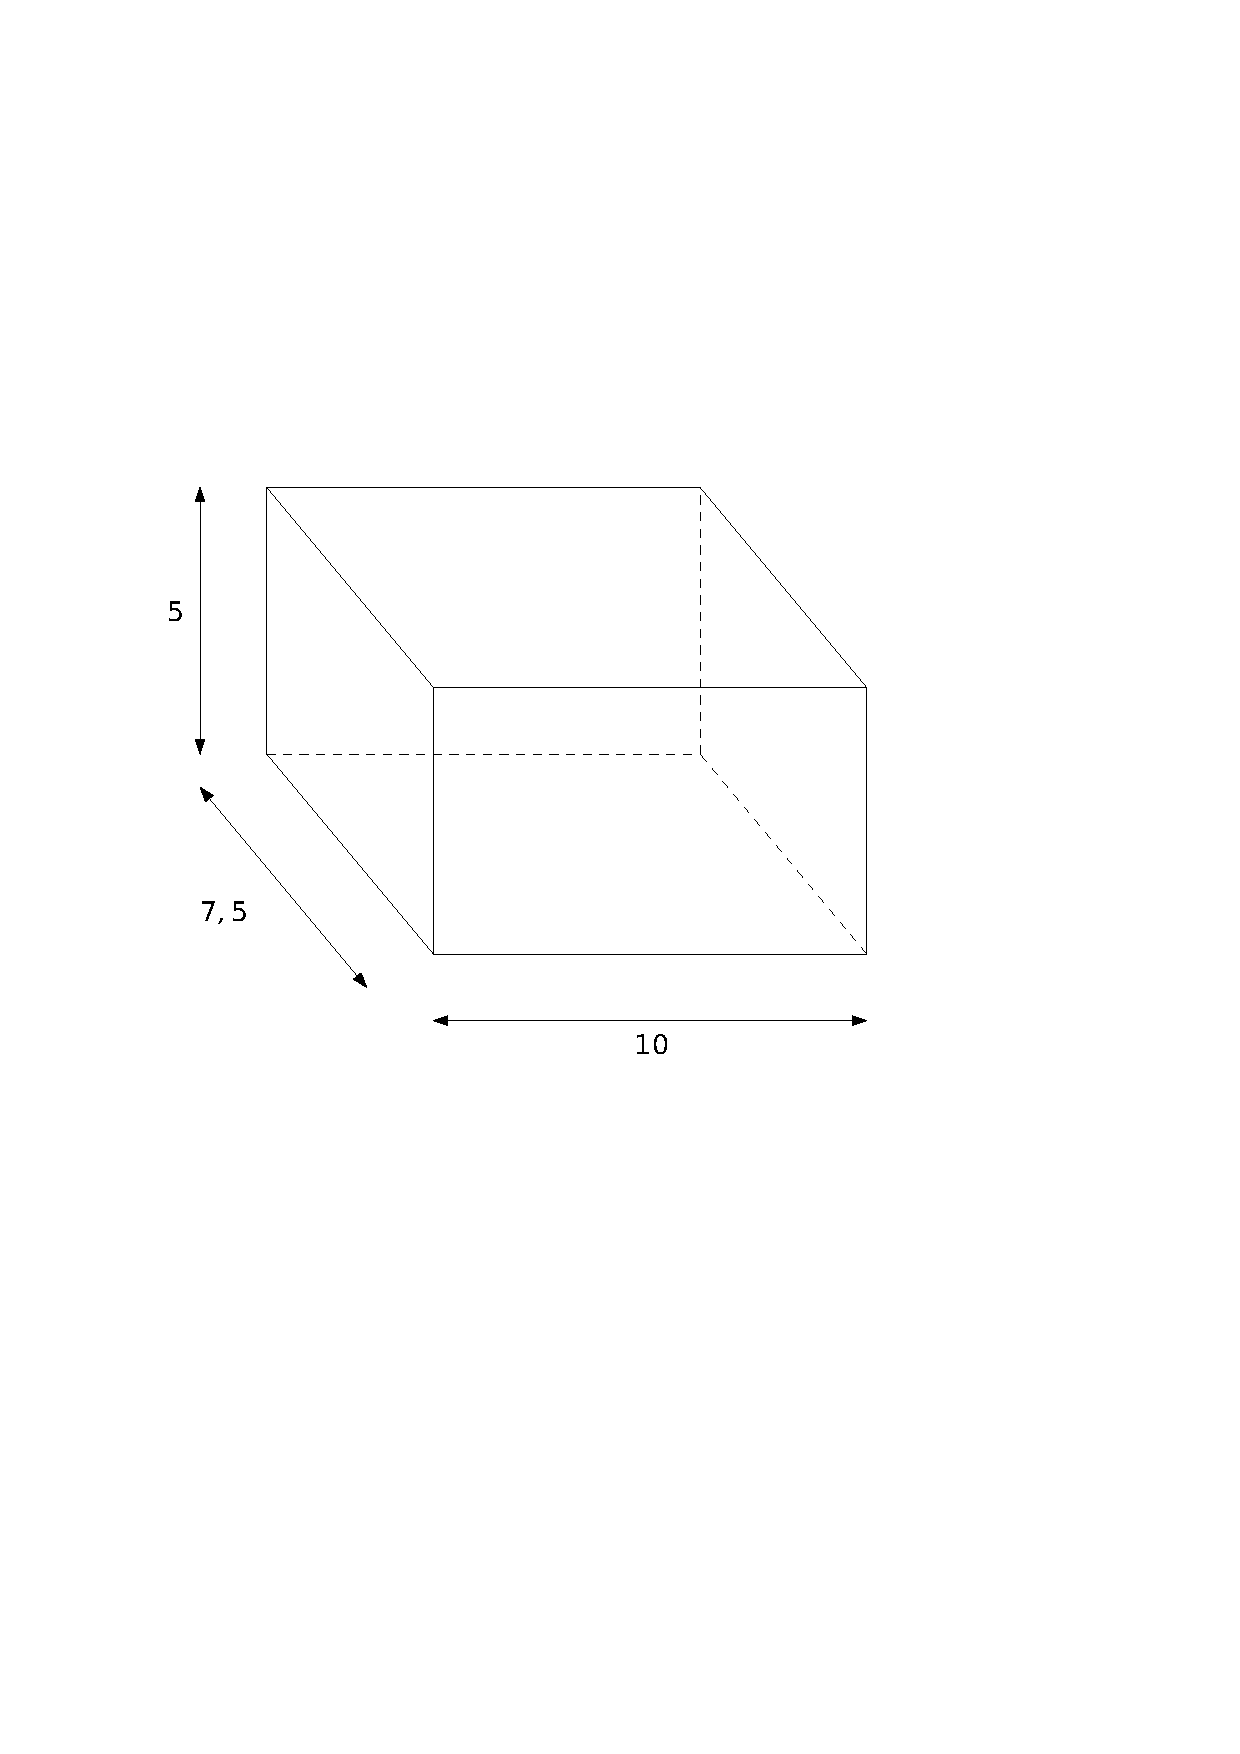
\includegraphics[scale=0.5]{media/gm-02/pave3.pdf}
    \task ~\\ 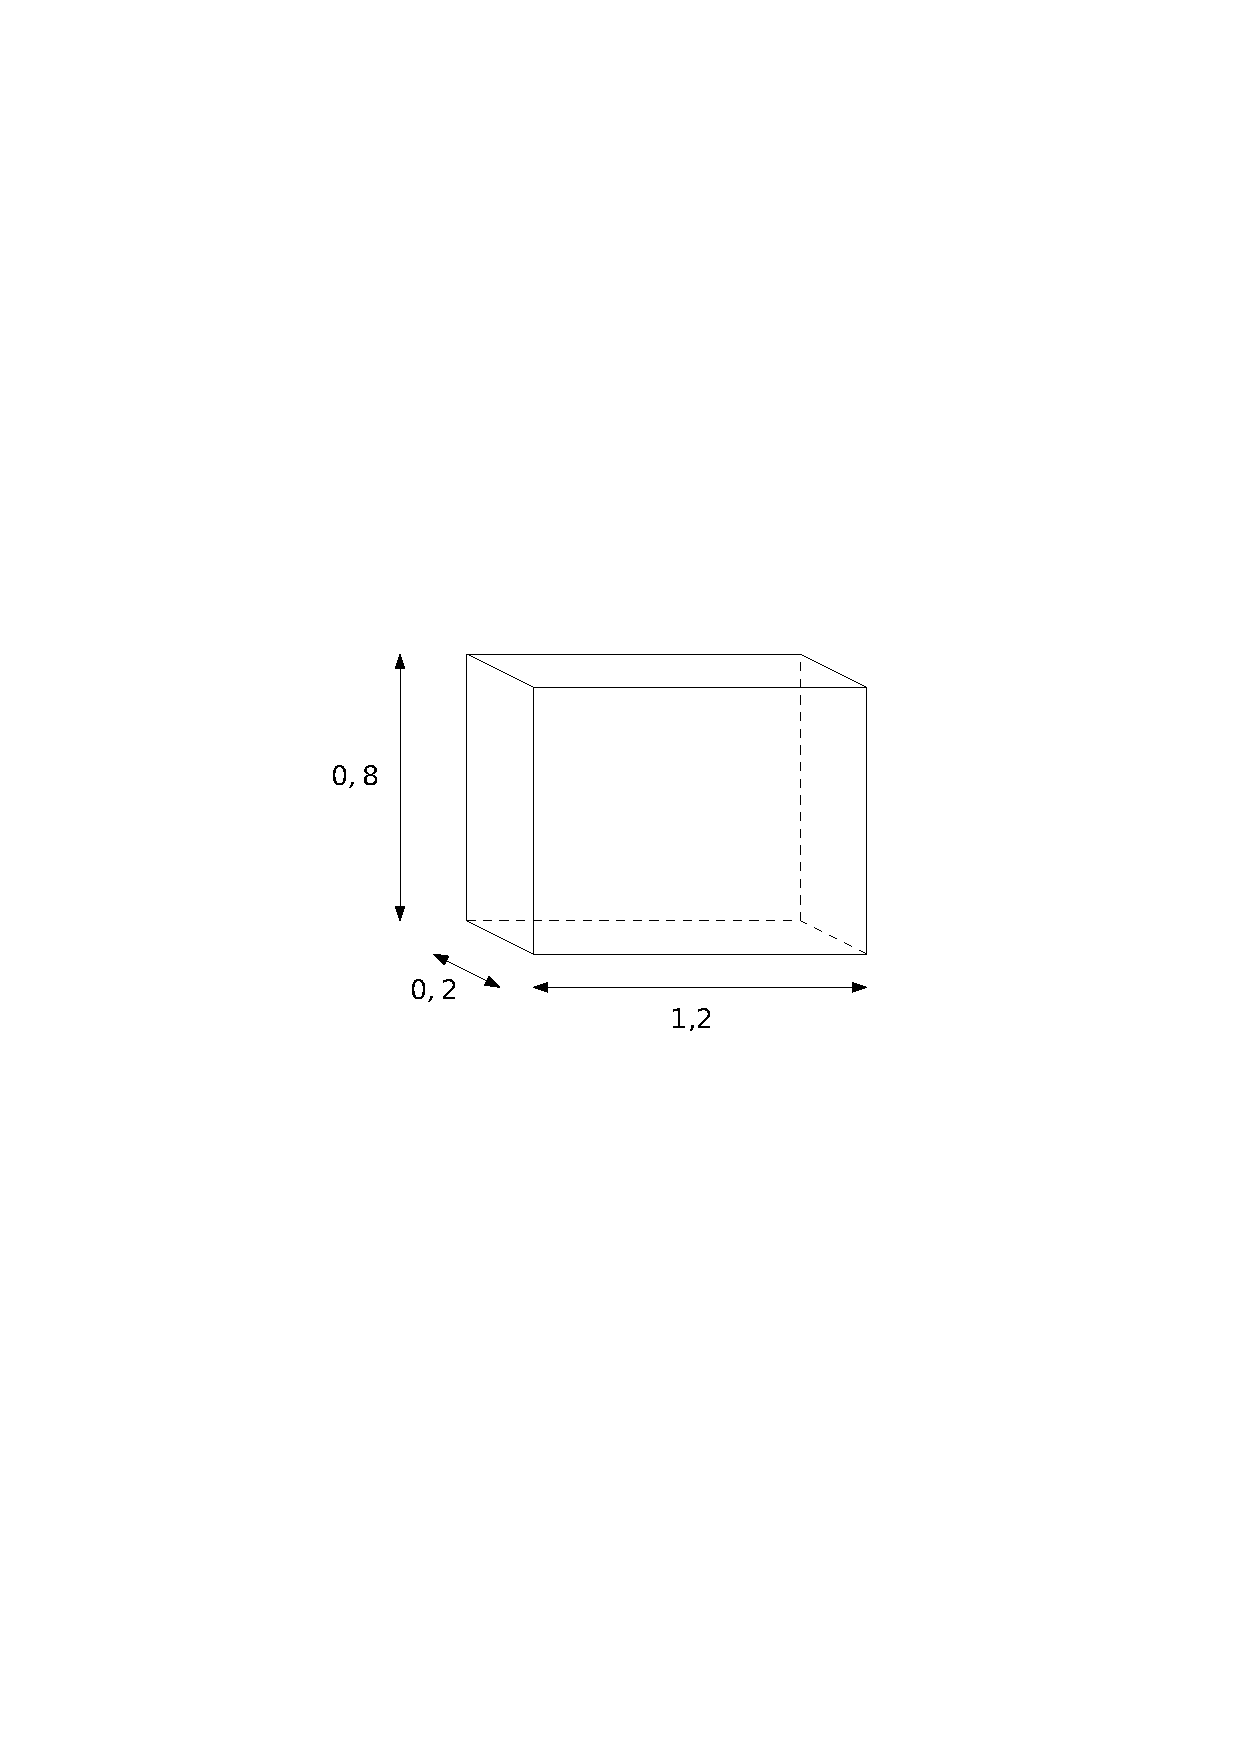
\includegraphics[scale=0.5]{media/gm-02/pave4.pdf}
\end{tasks}
}{1}
\end{exo}

\begin{exol}{GM54}{154}{1}
\end{exol}
\begin{exol}{GM55}{154}{1}
\end{exol}

\begin{exo}{
Calcule l'aire totale des pavés droits dont les développements sont représentés ci-dessous. Toutes les mesures sont exprimées en $\tunit{}{\kilo m}$.
\begin{tasks}(2)
    \task ~\\ 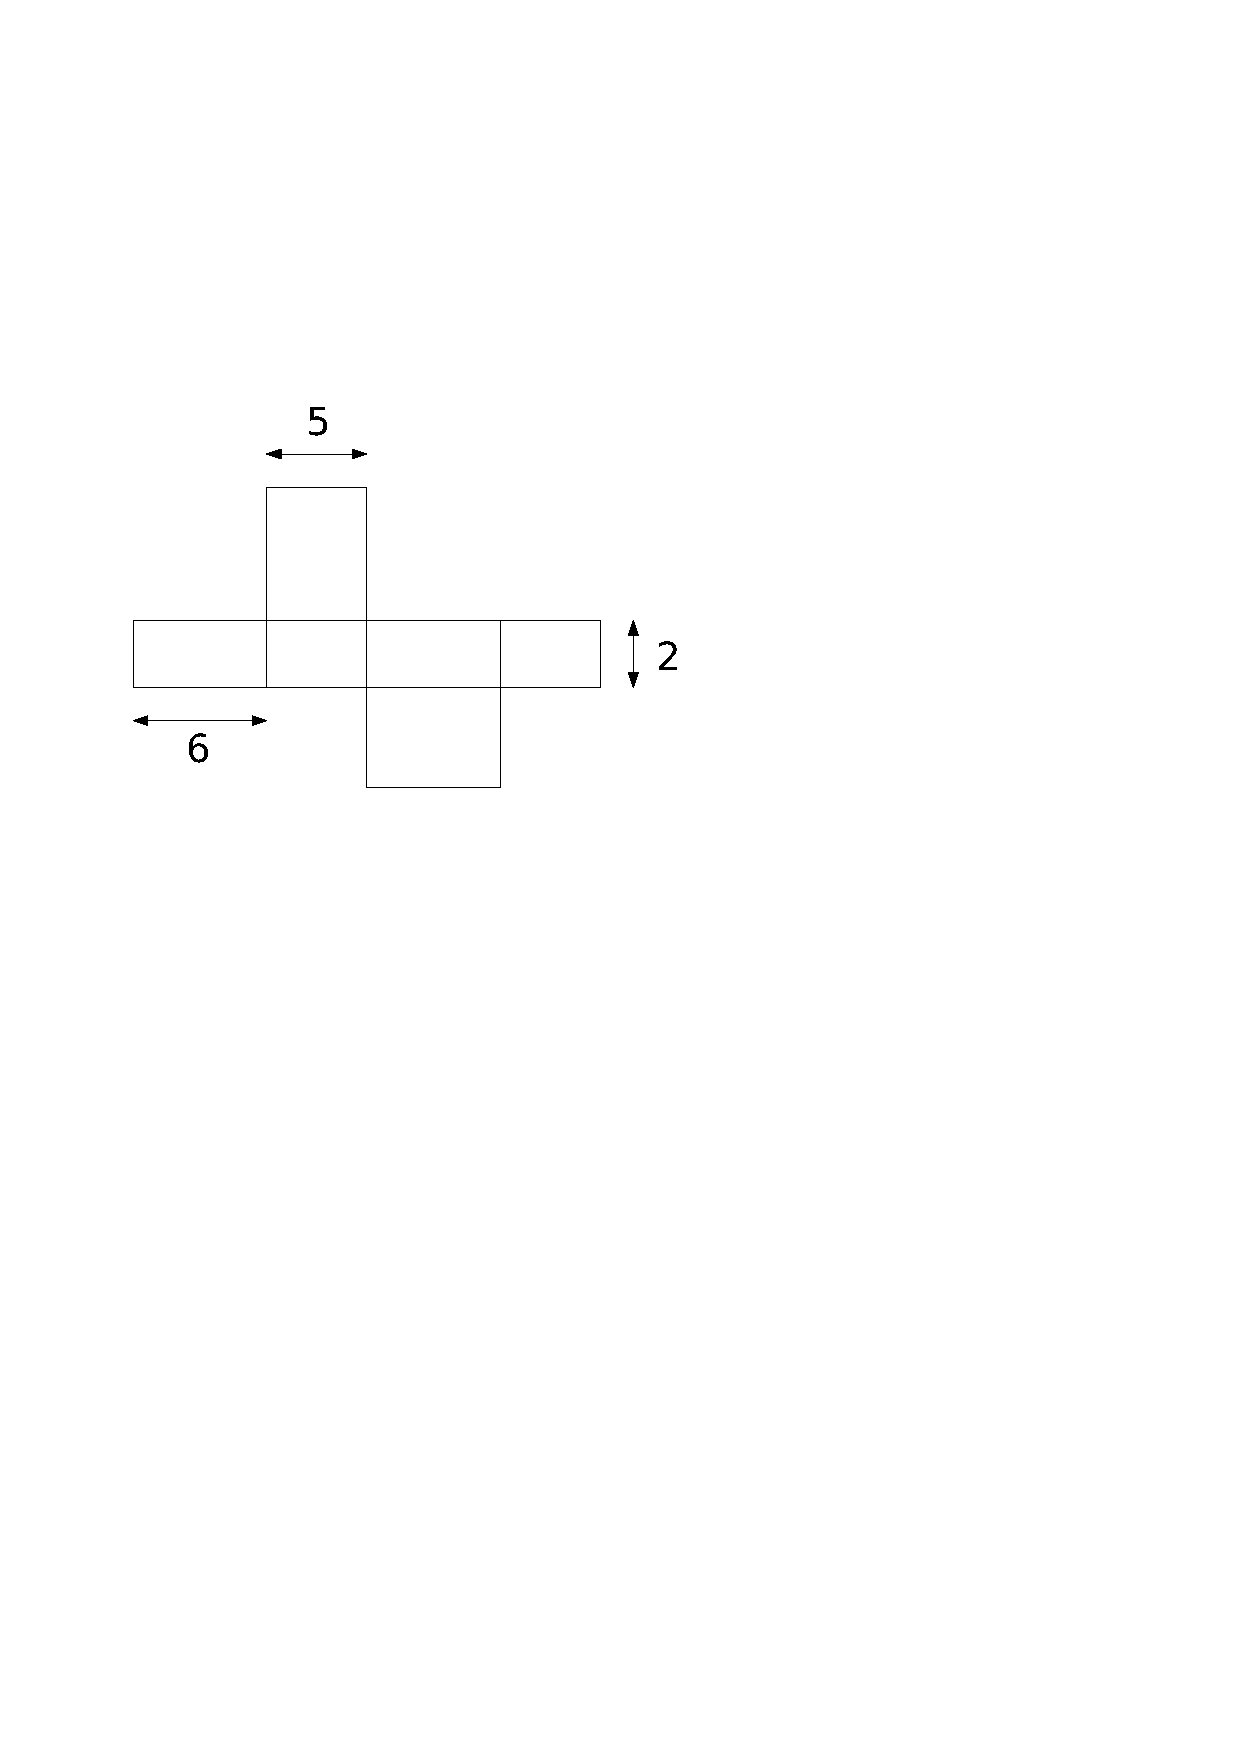
\includegraphics[scale=0.5]{media/gm-02/pave1-2.pdf}
    \task ~\\ 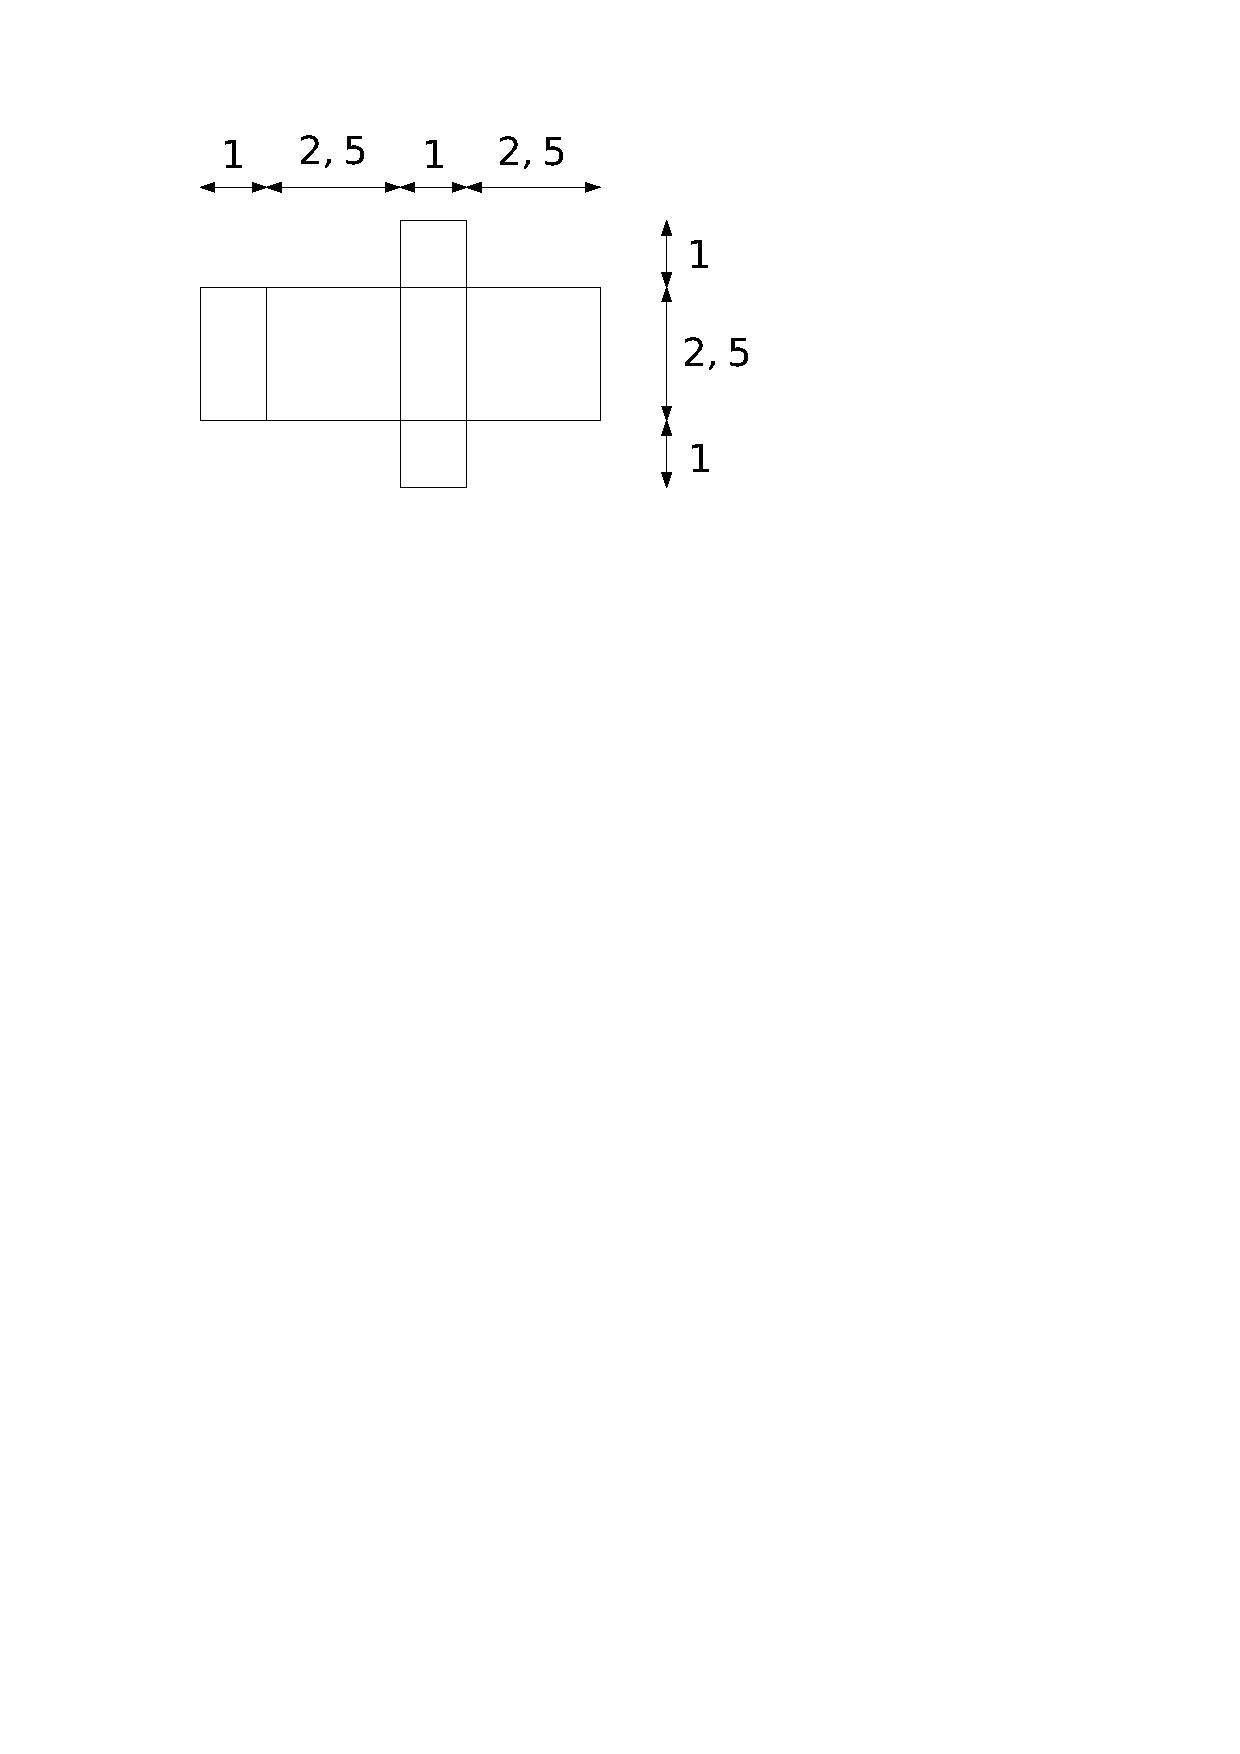
\includegraphics[scale=0.5]{media/gm-02/pave2-2.pdf}
    %\task ~\\ 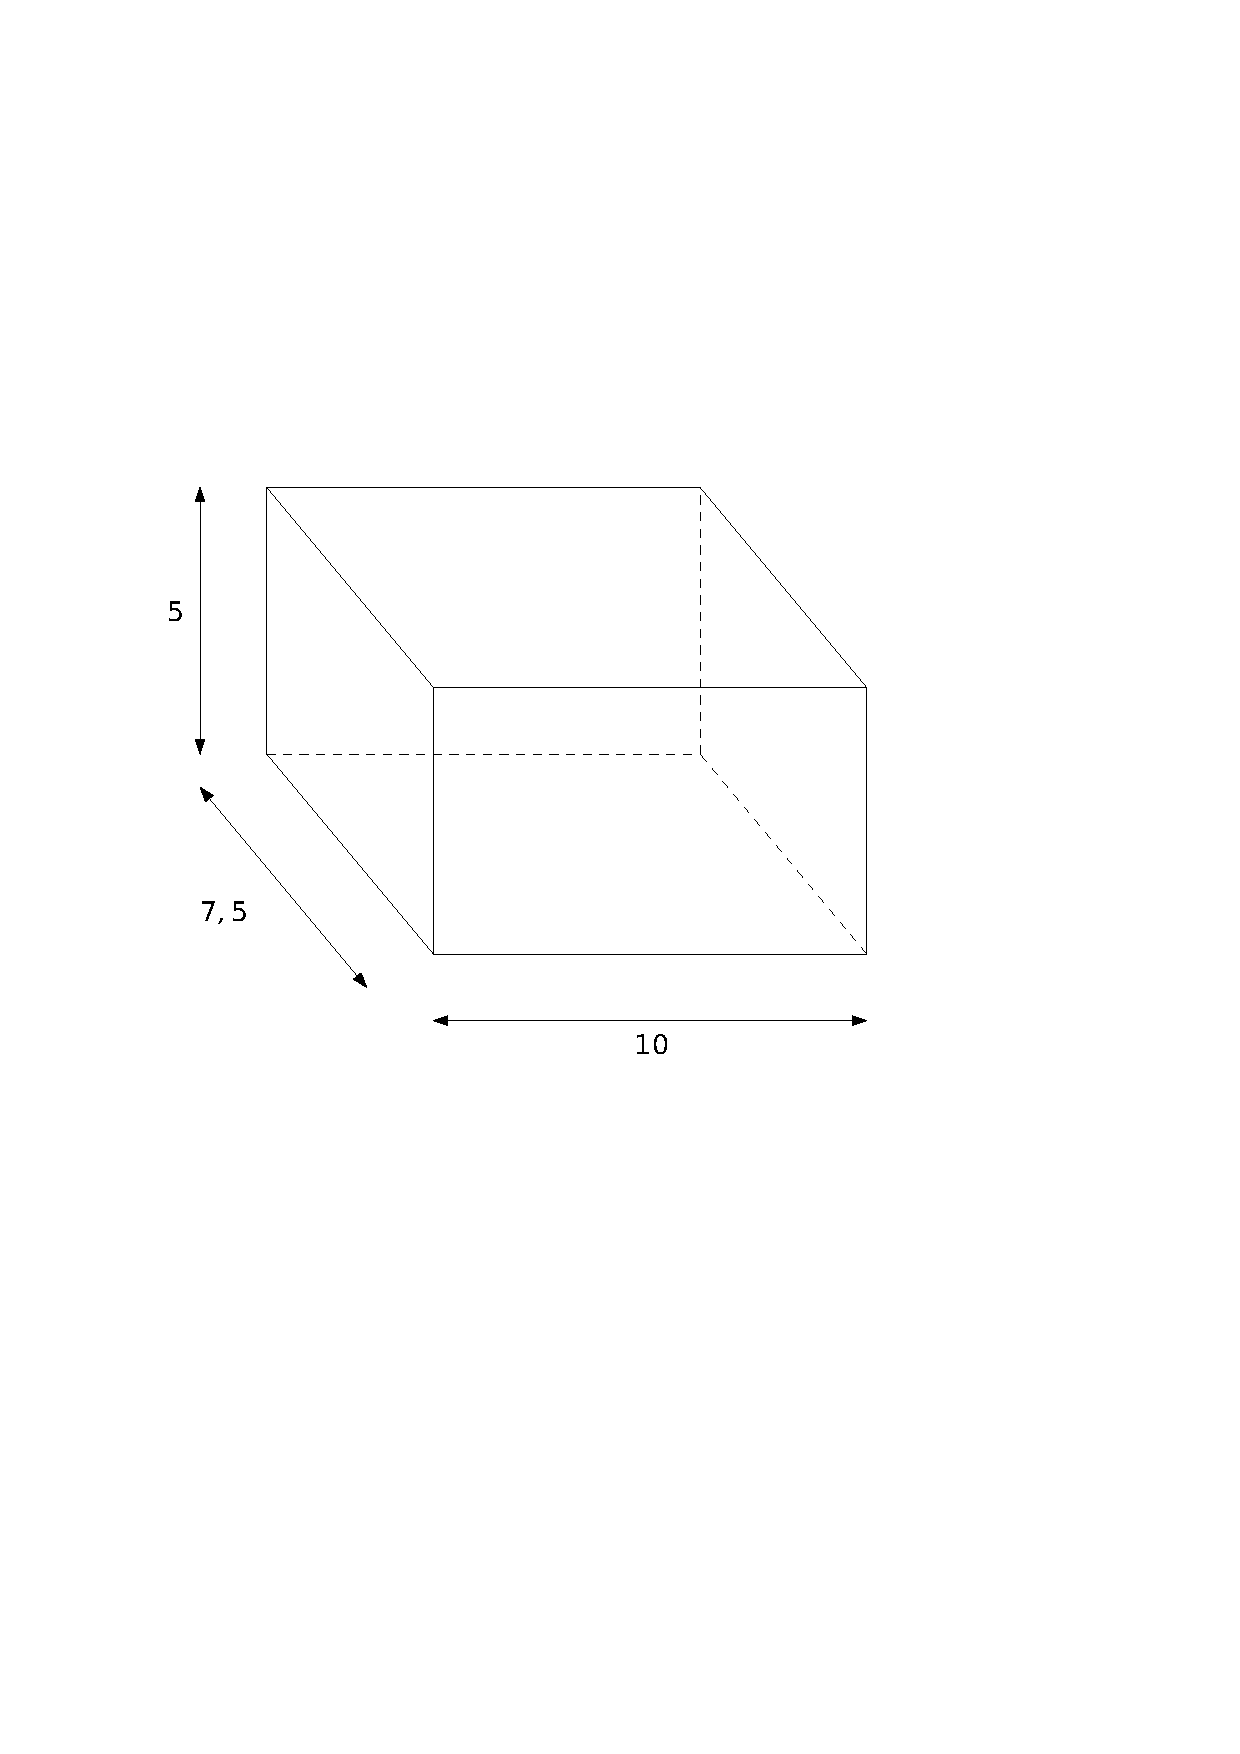
\includegraphics[scale=0.5]{media/gm-02/pave3.pdf}
    %\task ~\\ 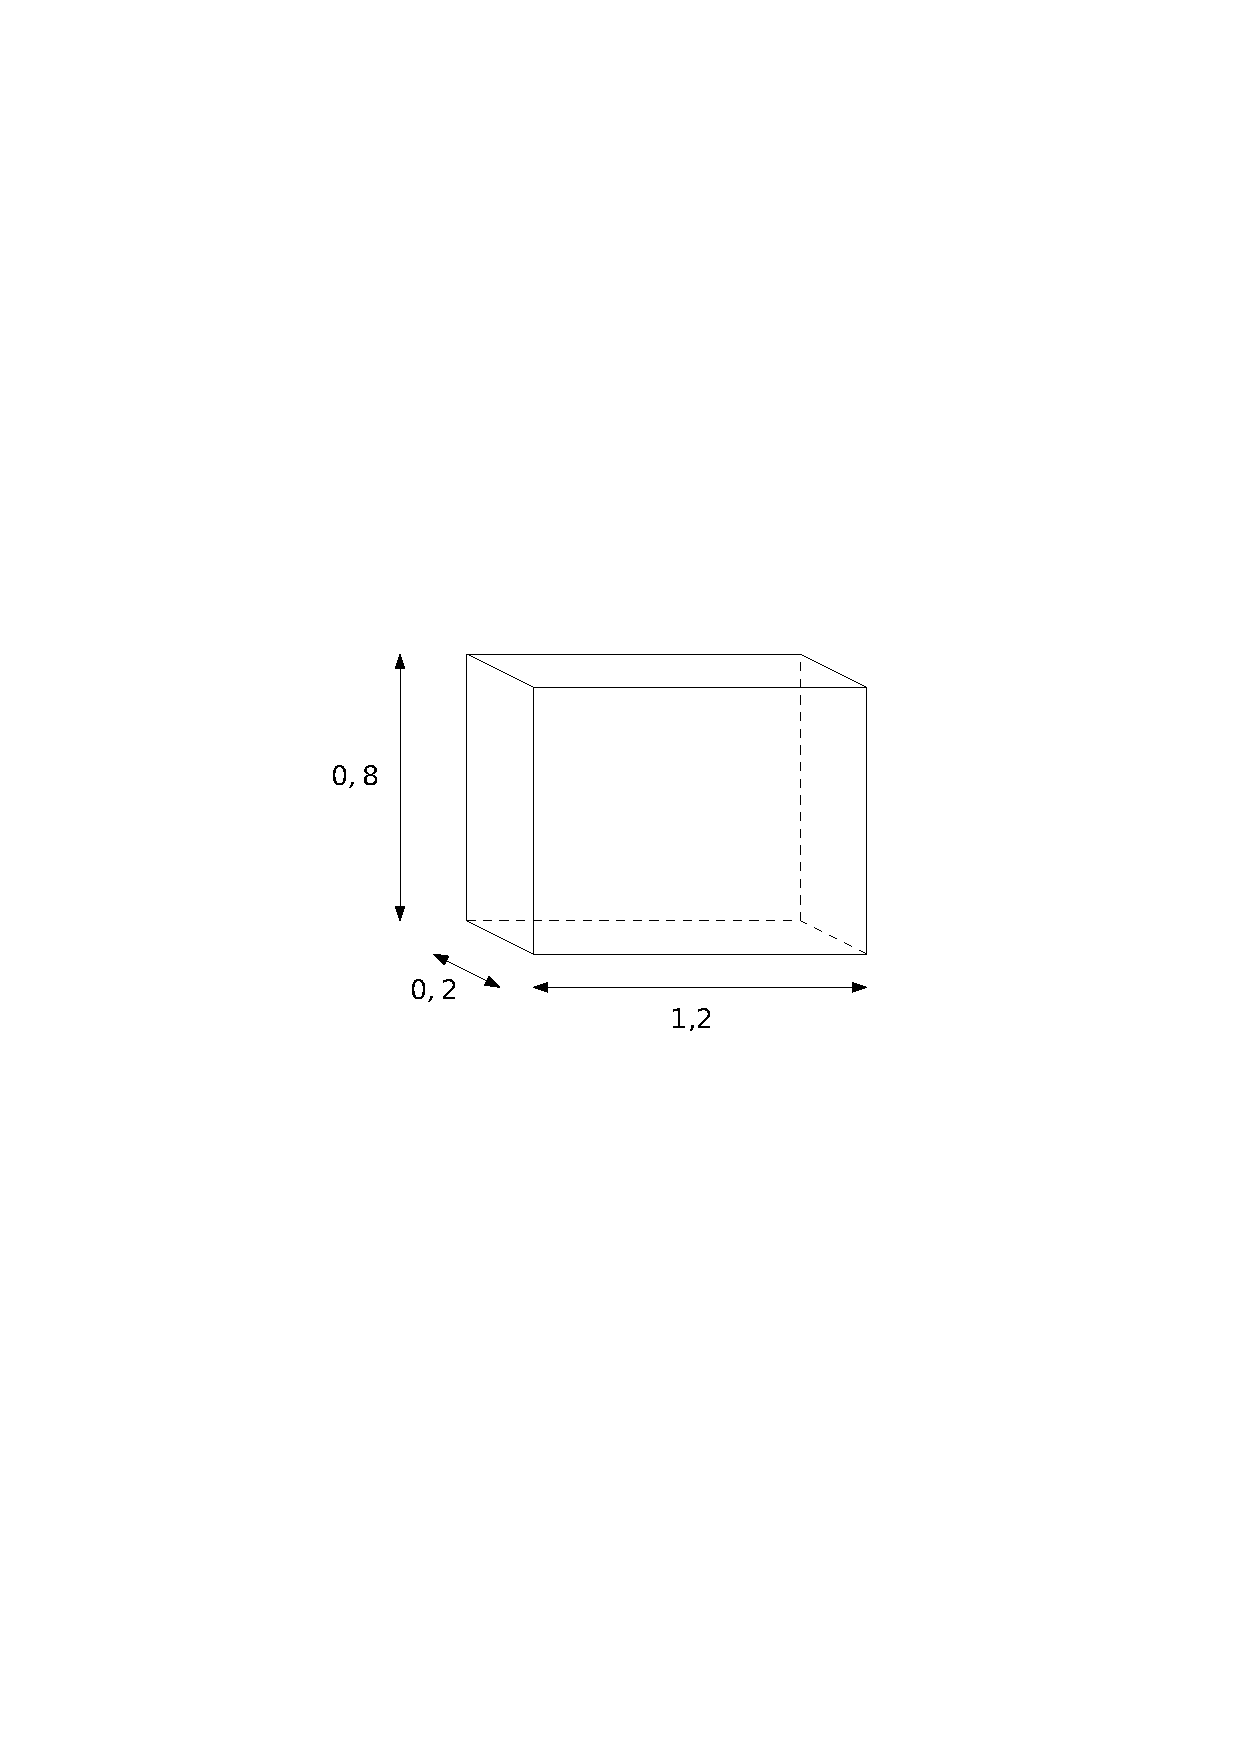
\includegraphics[scale=0.5]{media/gm-02/pave4.pdf}
\end{tasks}
}{1}   
\end{exo}

\begin{resolu}{Calculer l'aire totale d'un pavé droit}{
Calcule l'aire totale du pavé droit ci-dessous. Toutes les mesures sont exprimées en $\tunit{}{\centi m}$.
\begin{center}
    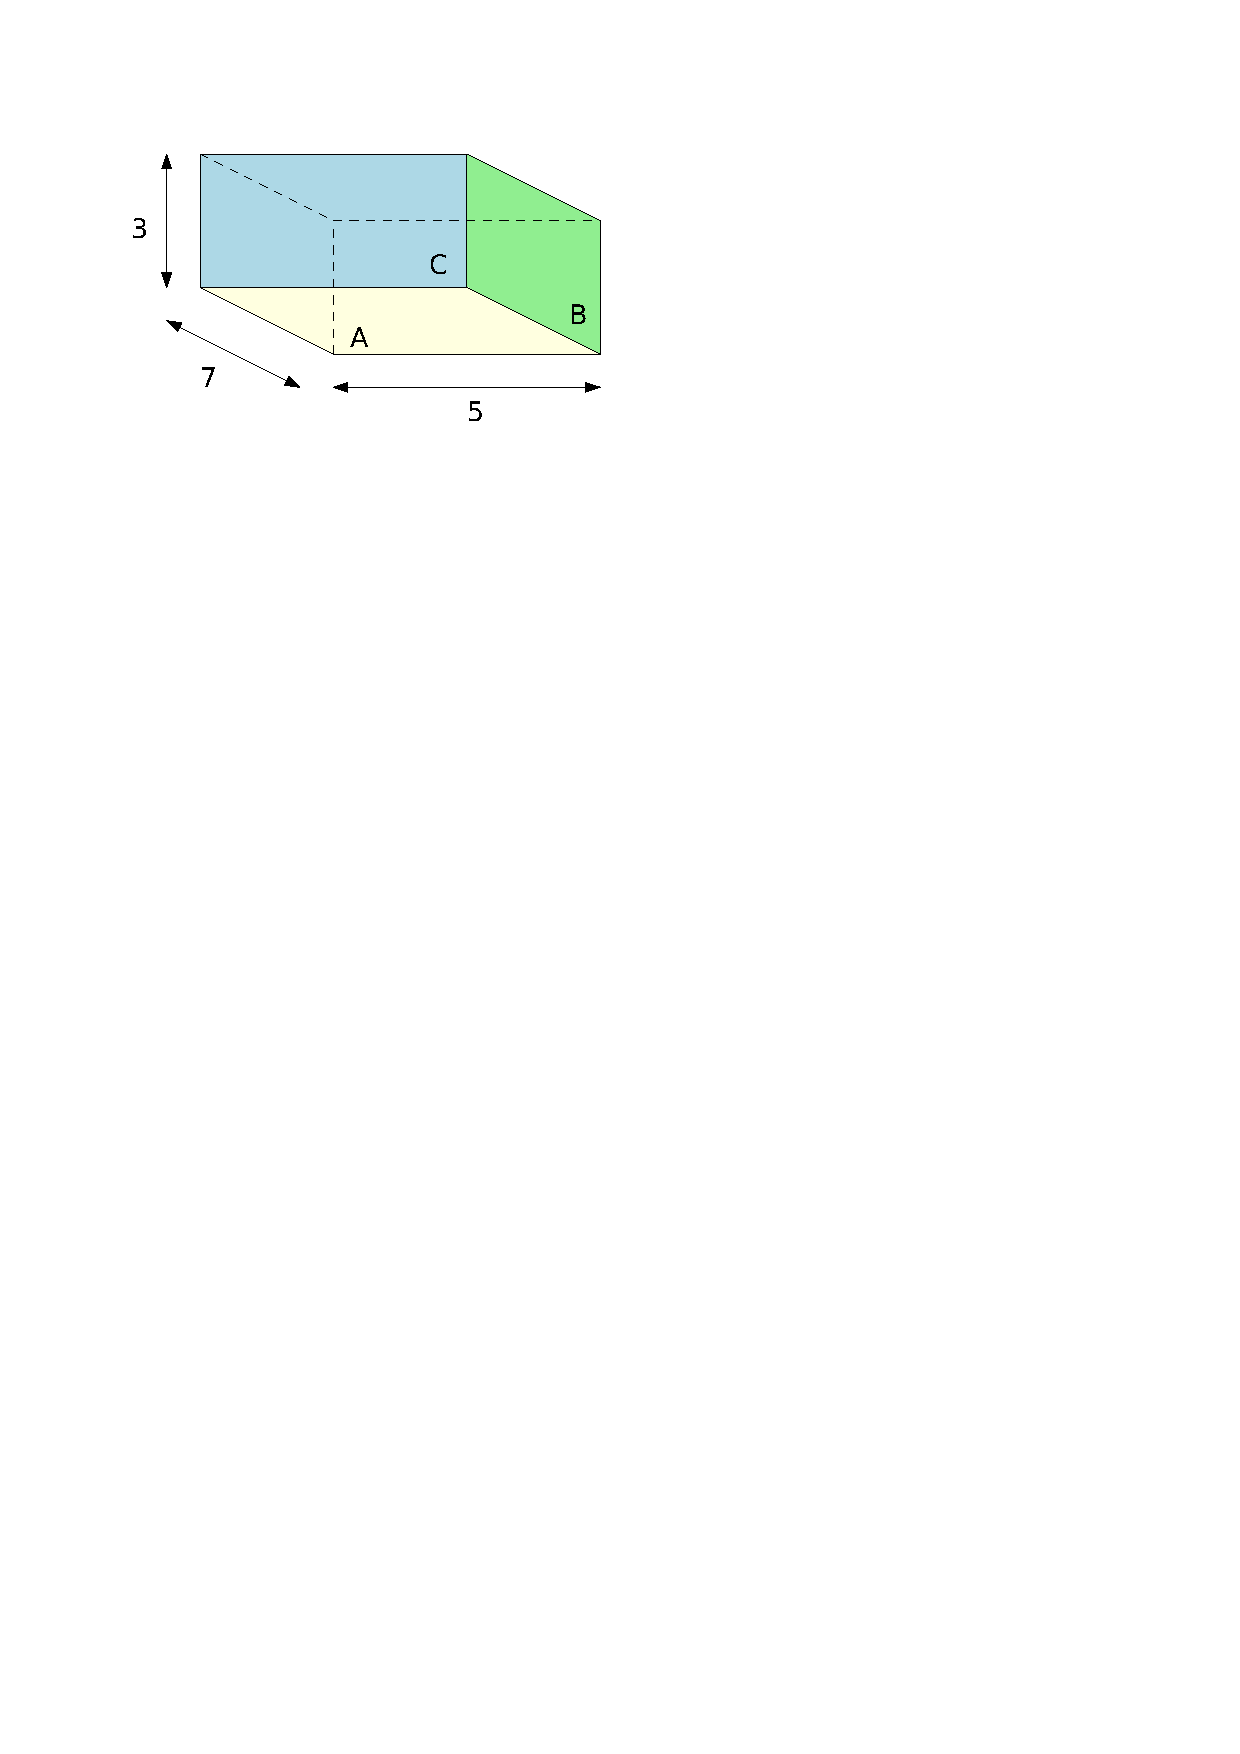
\includegraphics[scale=1]{media/gm-02/resolu-pave-droit.pdf}
\end{center}
\begin{enumerate}
    \item Un pavé droit possède trois paires de faces rectangulaires. Identifie leurs dimensions. 

    
    \item Calcule l'aire de chaque face.

    $\mathrm{Aire}_{\mathrm{~rectangle~A}}=7\cdot5=35$

    $\mathrm{Aire}_{\mathrm{~rectangle~B}}=7\cdot3=21$

    $\mathrm{Aire}_{\mathrm{~rectangle~C}}=3\cdot5=15$
    
    \item Additionne les résultats obtenus.
    \begin{align*}
        \mathrm{Aire}_{\mathrm{~totale}}&=2\cdot \mathrm{Aire}_{\mathrm{~rect.~A}} + 2\cdot \mathrm{Aire}_{\mathrm{~rect.~B}} + 2\cdot \mathrm{Aire}_{\mathrm{~rect.~C}}\\
        &= 2\cdot 35 + 2\cdot21 + 2\cdot15=70+42+30\\
        &=\tunit{142}{\centi m^2}   
    \end{align*}
    
\end{enumerate}
}{1}    
\end{resolu}


%aire totale cube, pavé droit (+ conversion d'unité)
\begin{exo}{
Calcule l'aire totale des pavés droits représentés ci-dessous. Toutes les mesures sont exprimées en $\tunit{}{\centi m}$.

\begin{tasks}(2)
    \task ~\\ 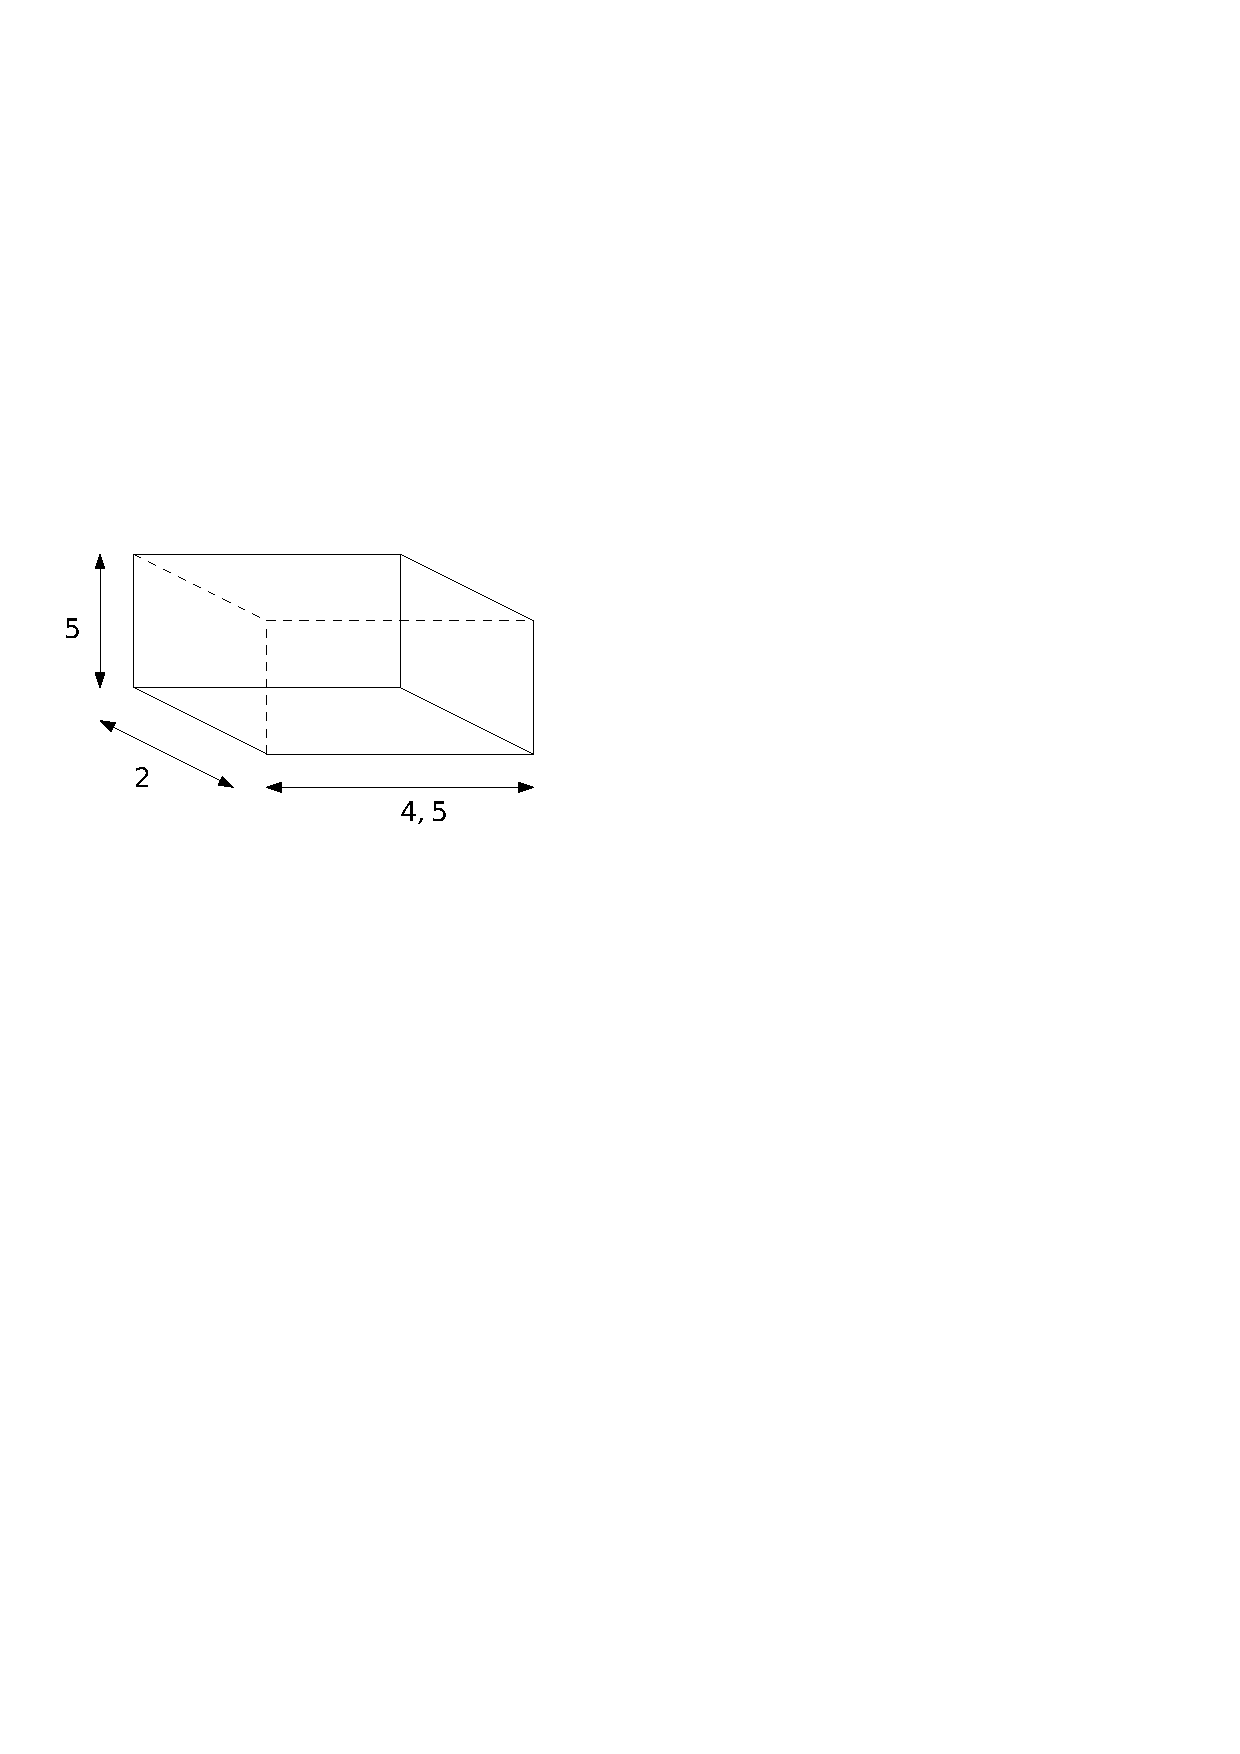
\includegraphics[scale=0.5]{media/gm-02/pave1.pdf}
    \task ~\\ 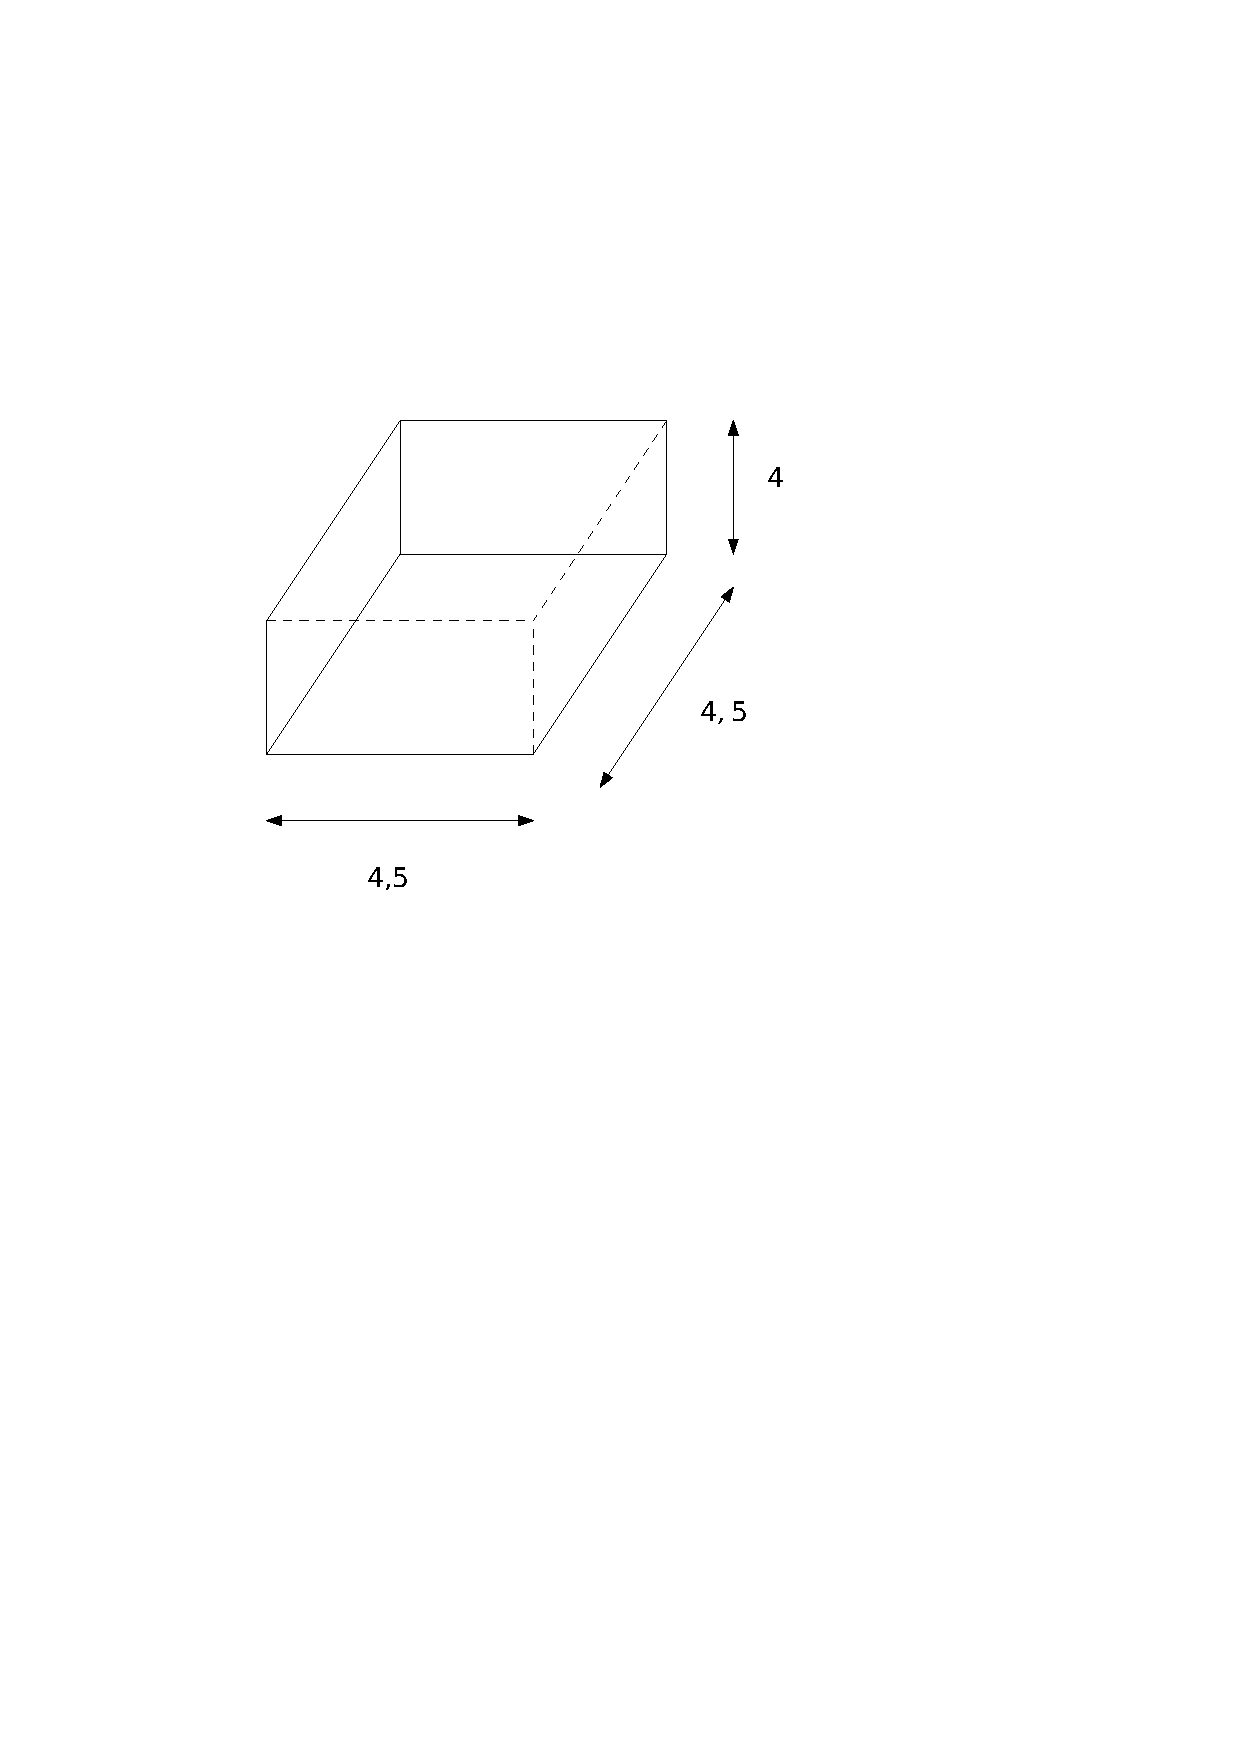
\includegraphics[scale=0.5]{media/gm-02/pave2.pdf}
    \task ~\\ 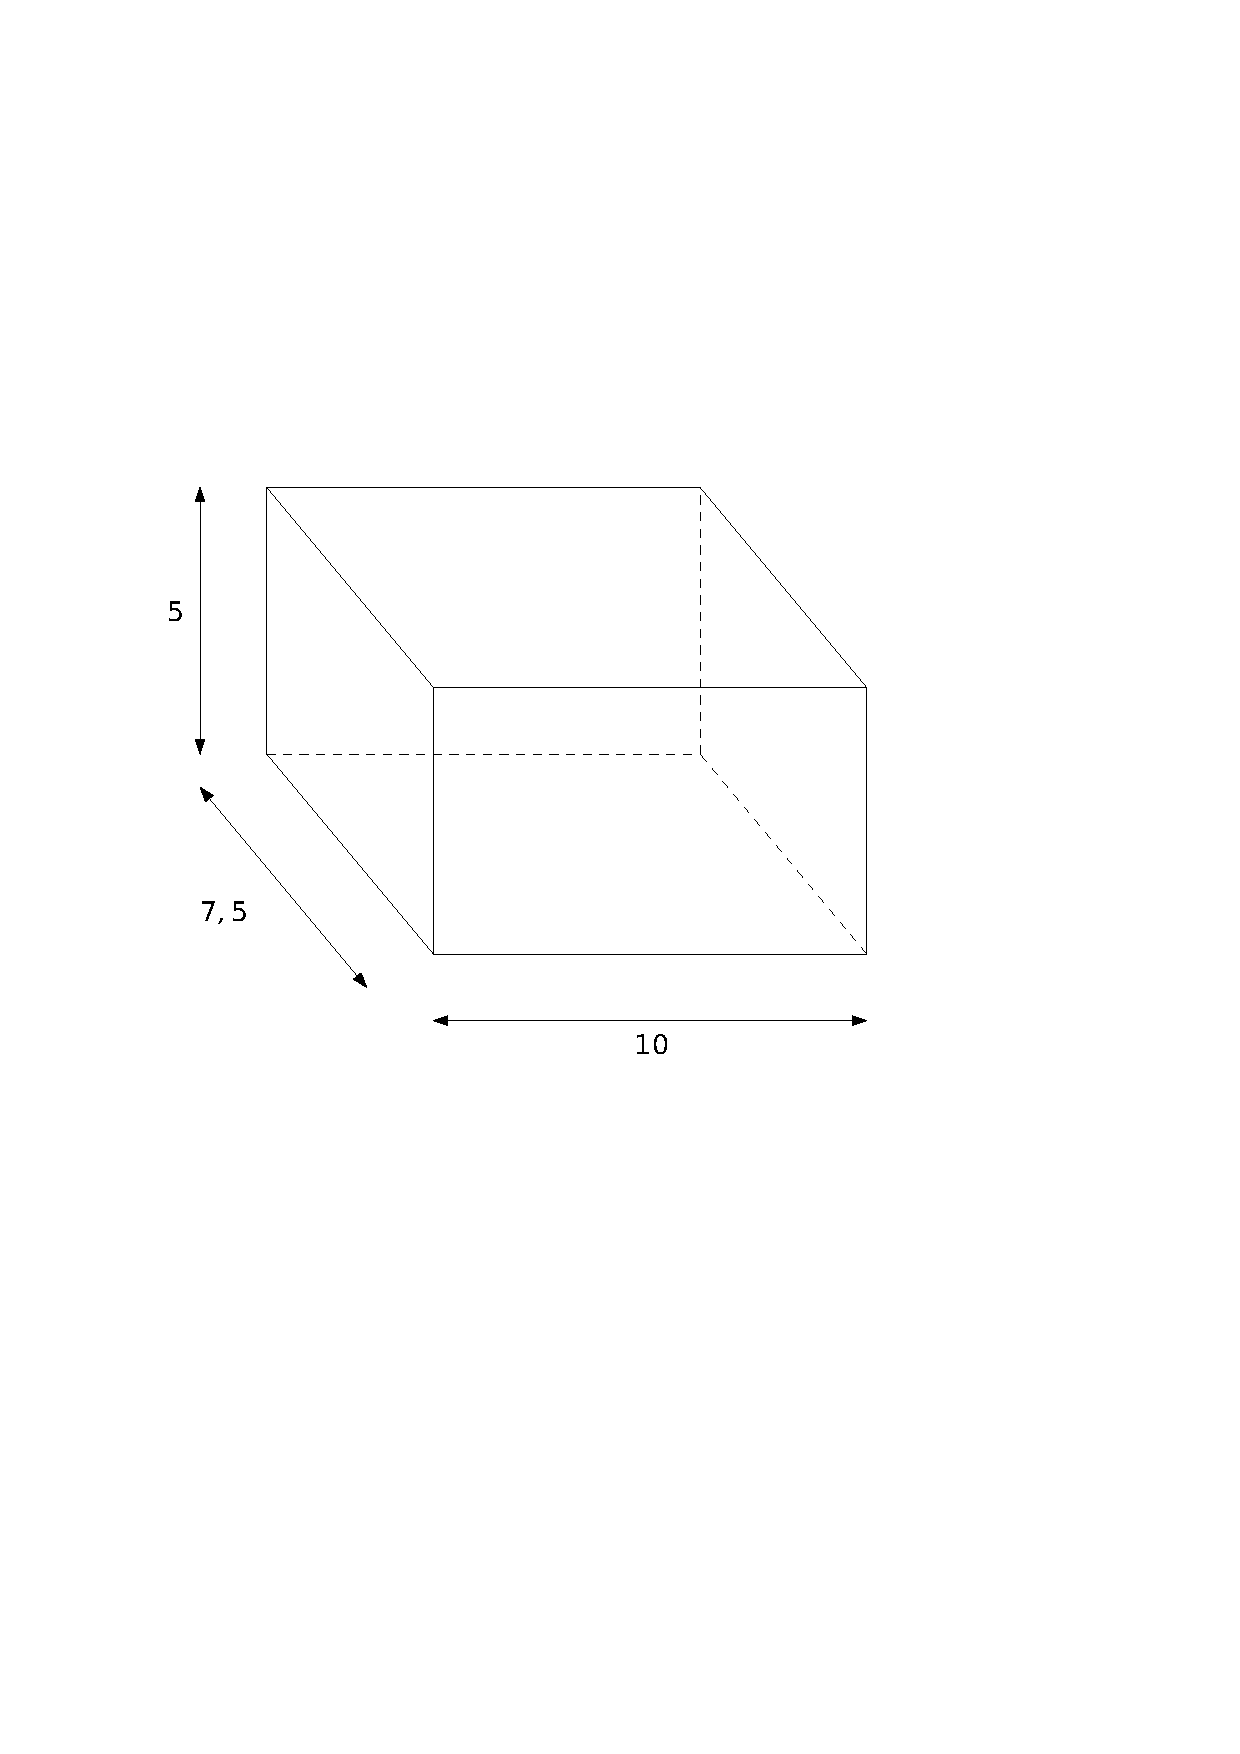
\includegraphics[scale=0.5]{media/gm-02/pave3.pdf}
    \task ~\\ 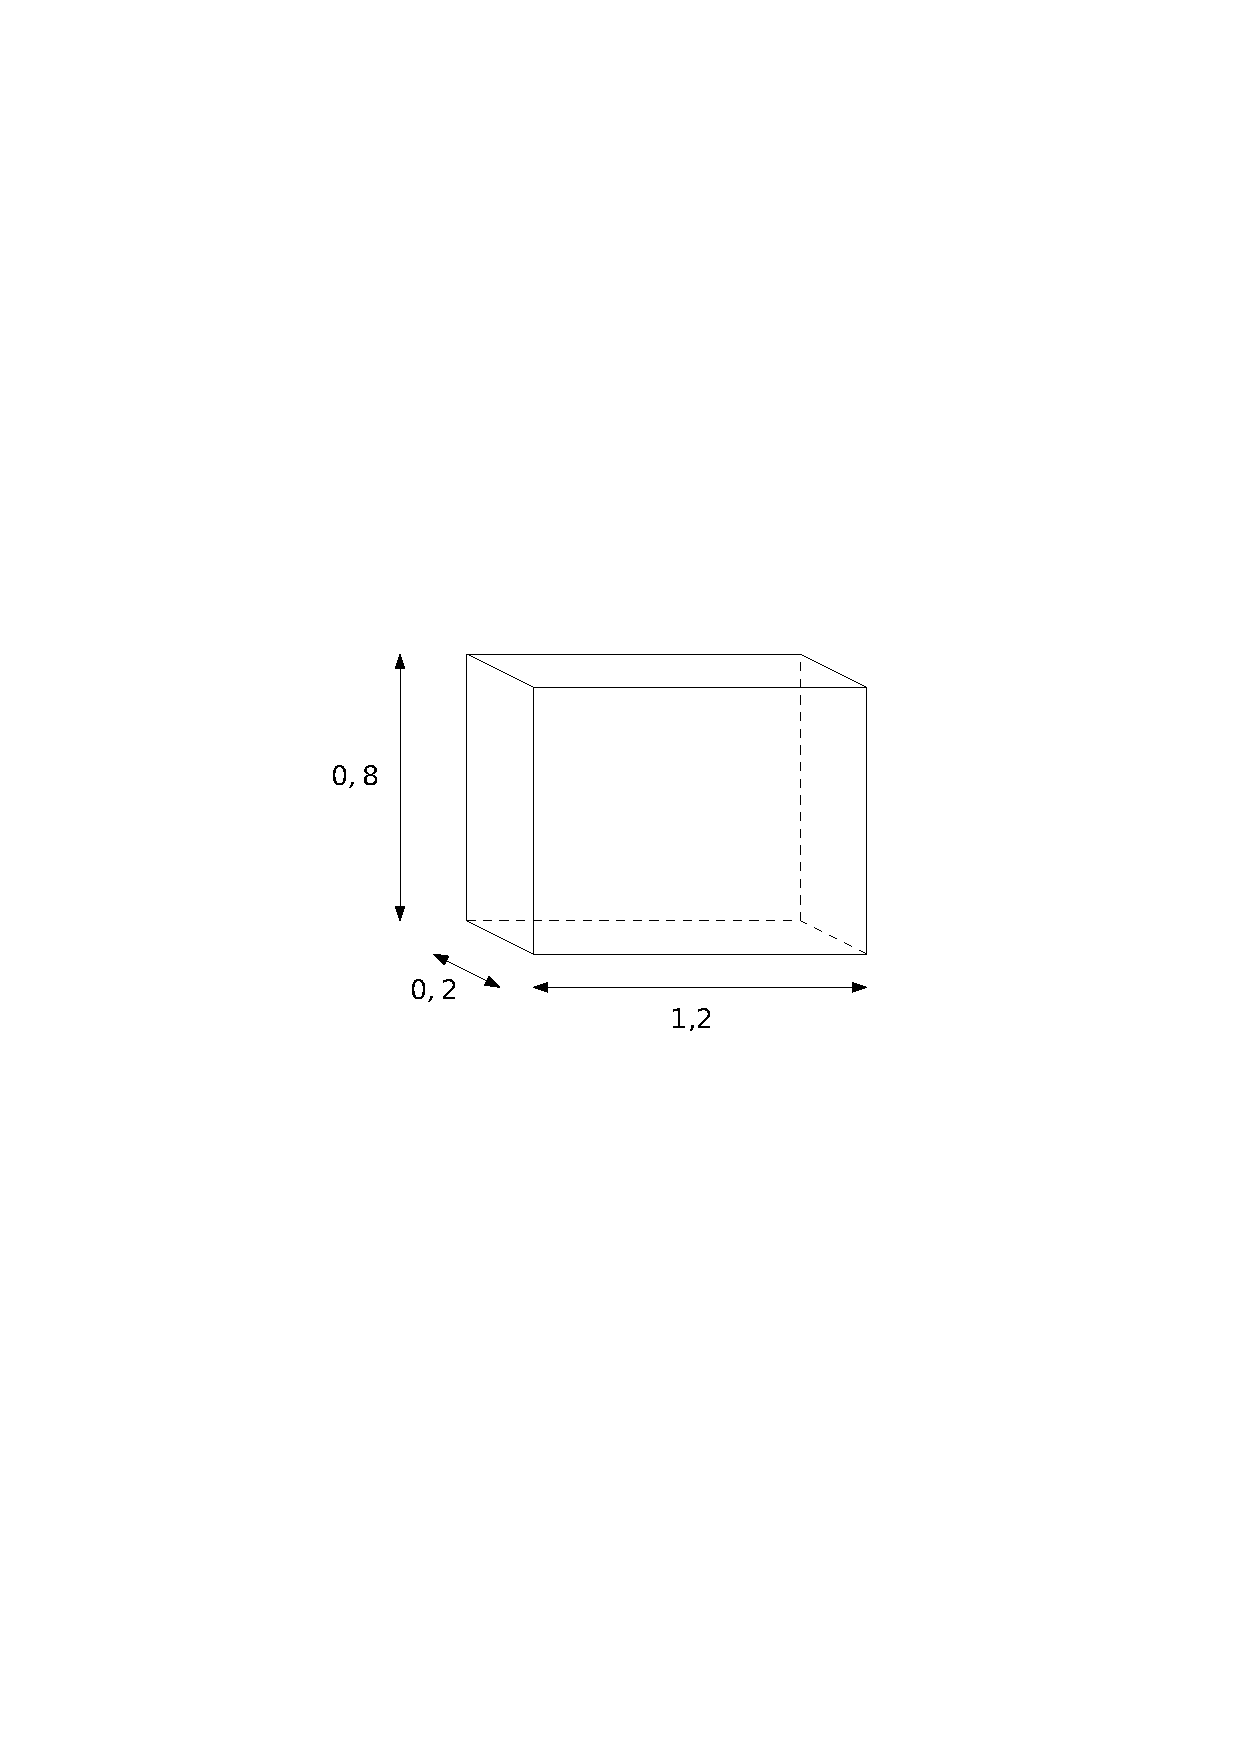
\includegraphics[scale=0.5]{media/gm-02/pave4.pdf}
\end{tasks}
}{1}
\end{exo}



%volume, aire totale, longueur pavés droits
\begin{exol}{GM60}{155}{2}
\end{exol}


%longueur manquante pavé droit
\begin{exol}{GM58}{154}{$\star$}
\end{exol}

%long manquante pavé droit
\begin{exof}{GM57}{199}{$\star$}
\end{exof}




% Minimiser aire totale pavé droit
\begin{exol}{GM64}{157}{2}
\end{exol}

% Minimiser aire totale pavé droit
\begin{exol}{GM59}{155}{2}
\end{exol}


\begin{exop}{
Calcule le volume des prismes droits représentés ci-dessous. Toutes les mesures sont exprimées en $\tunit{}{\centi m}$.

\begin{tasks}(2)
    \task ~\\ 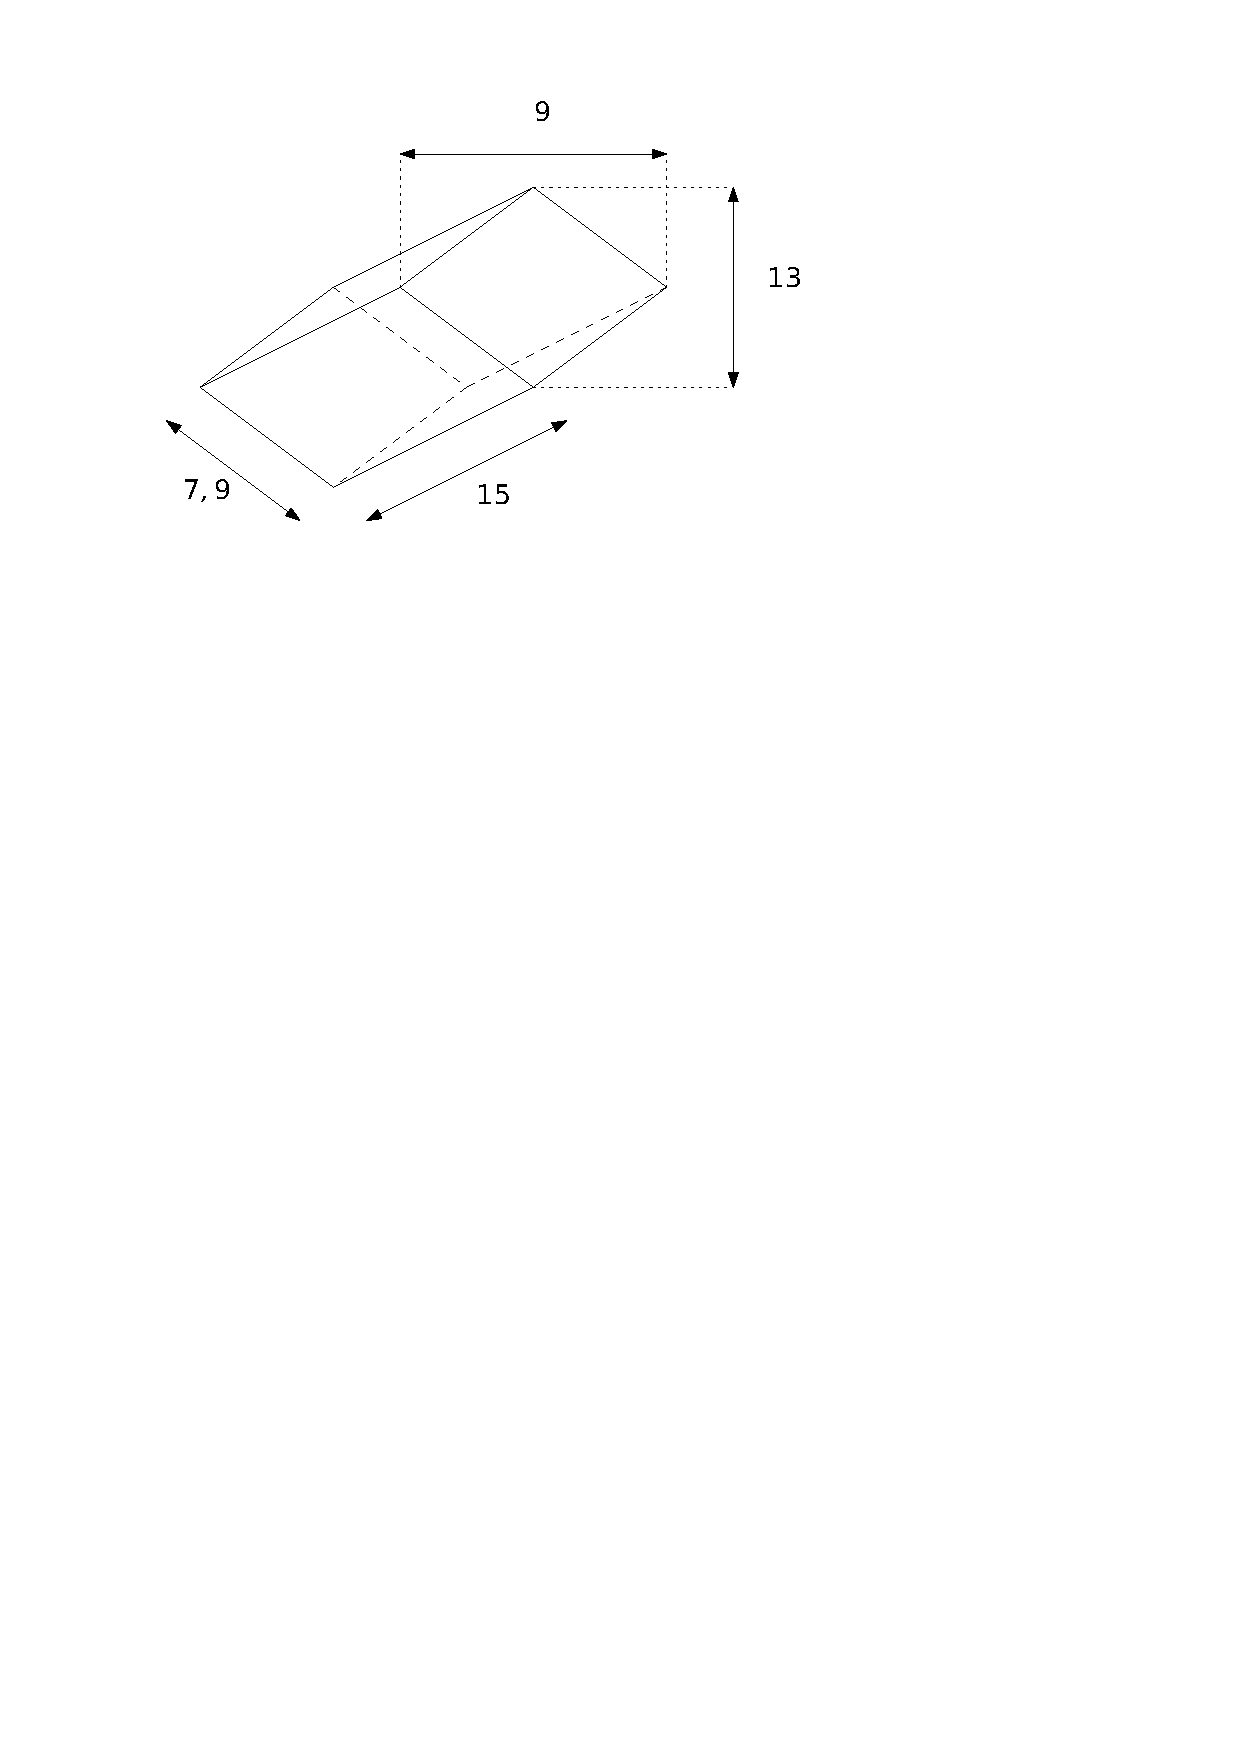
\includegraphics[scale=0.5]{media/gm-02/prisme-los.pdf}
    \task ~\\ 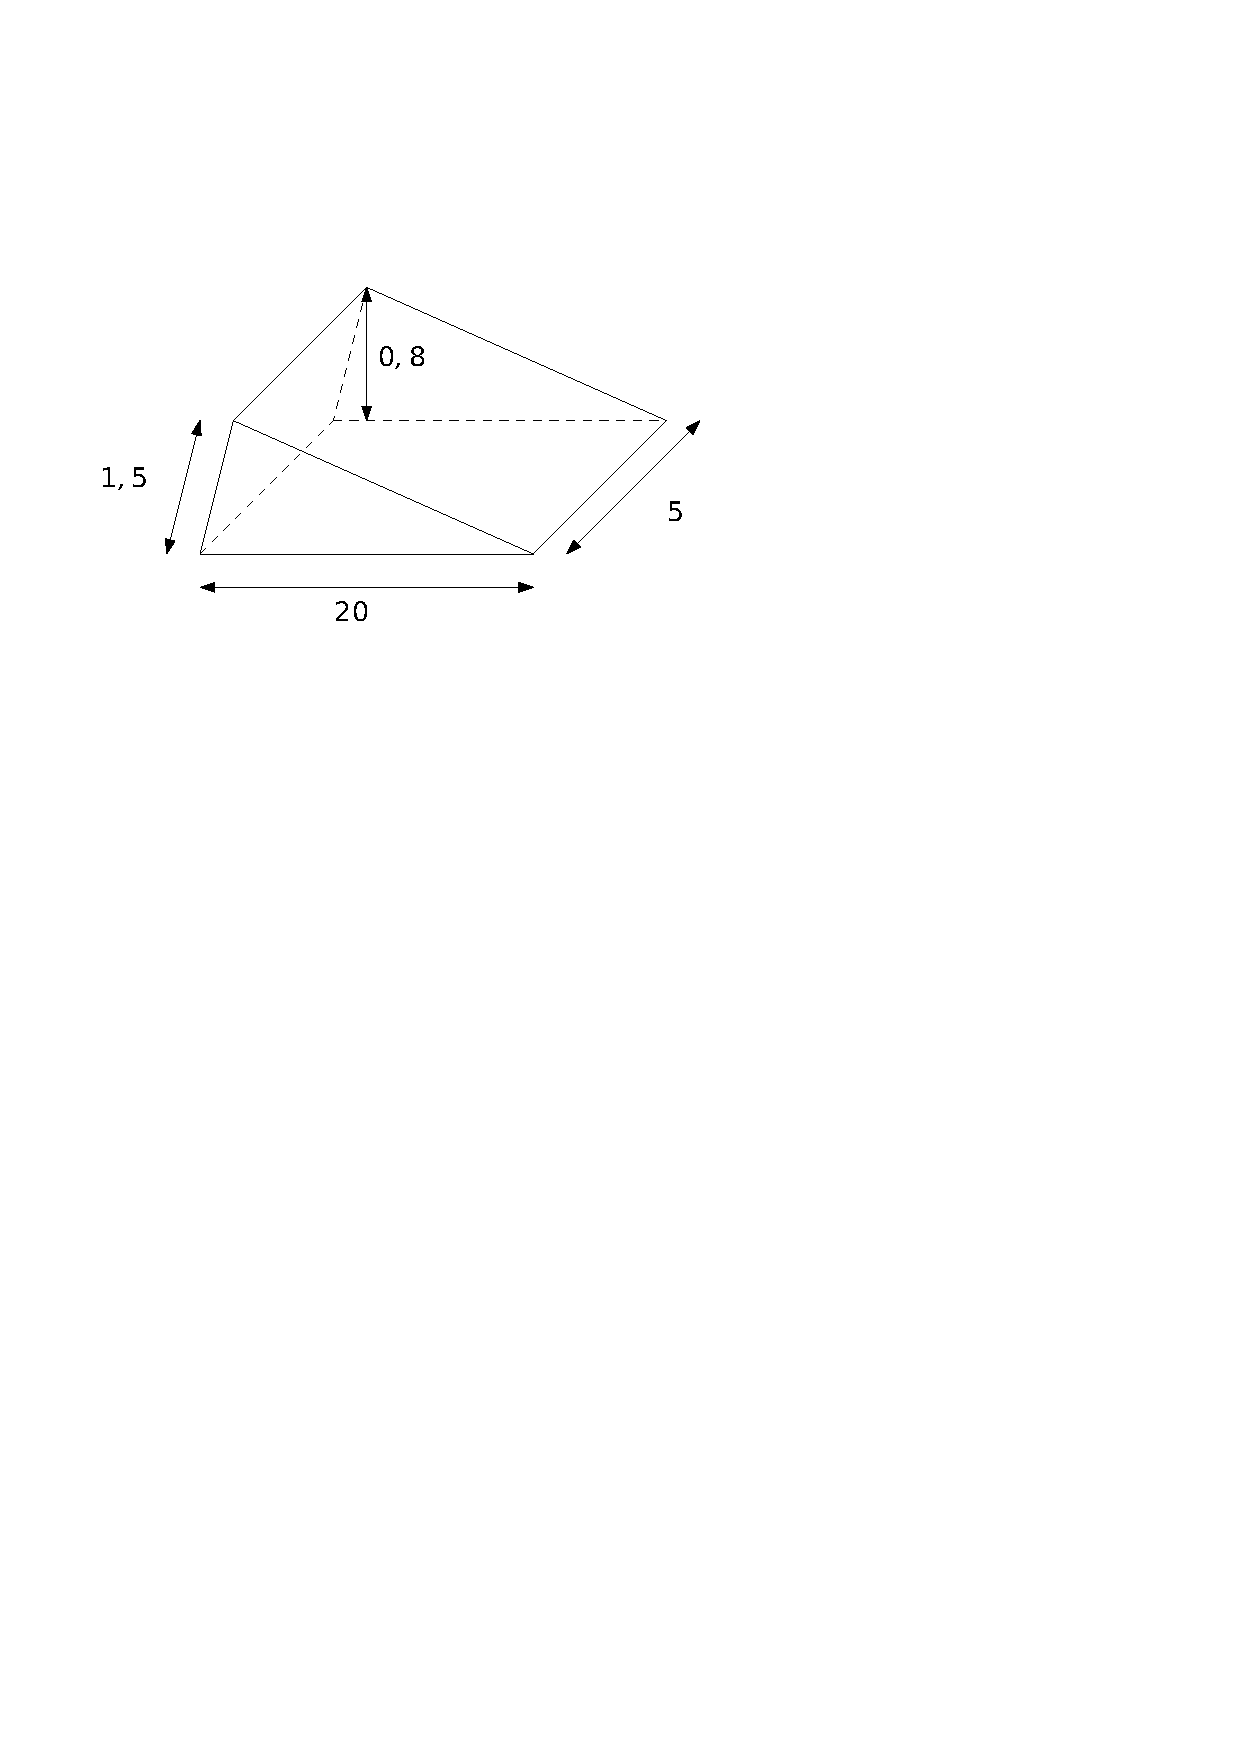
\includegraphics[scale=0.5]{media/gm-02/prisme-triang2.pdf}
    \task ~\\ 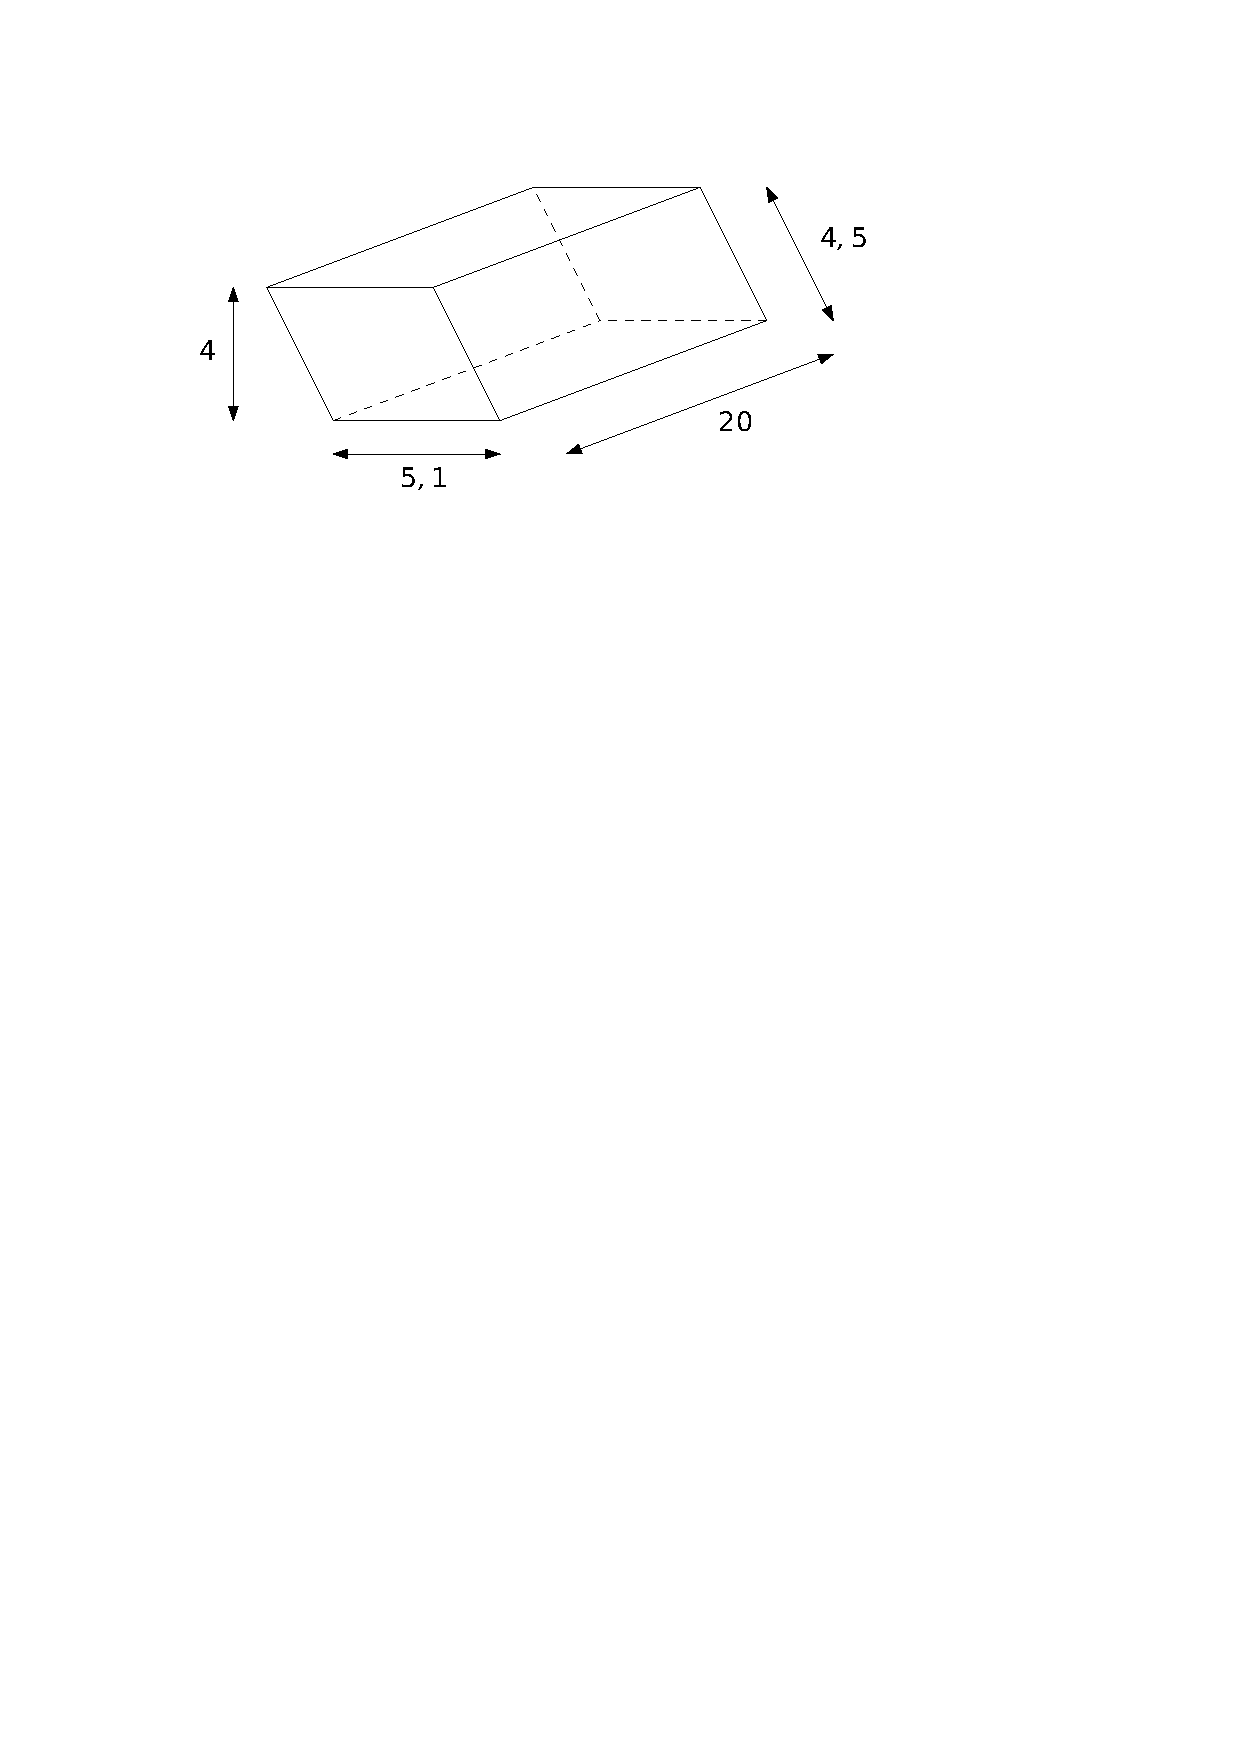
\includegraphics[scale=0.5]{media/gm-02/prisme-para.pdf}
    \task ~\\ 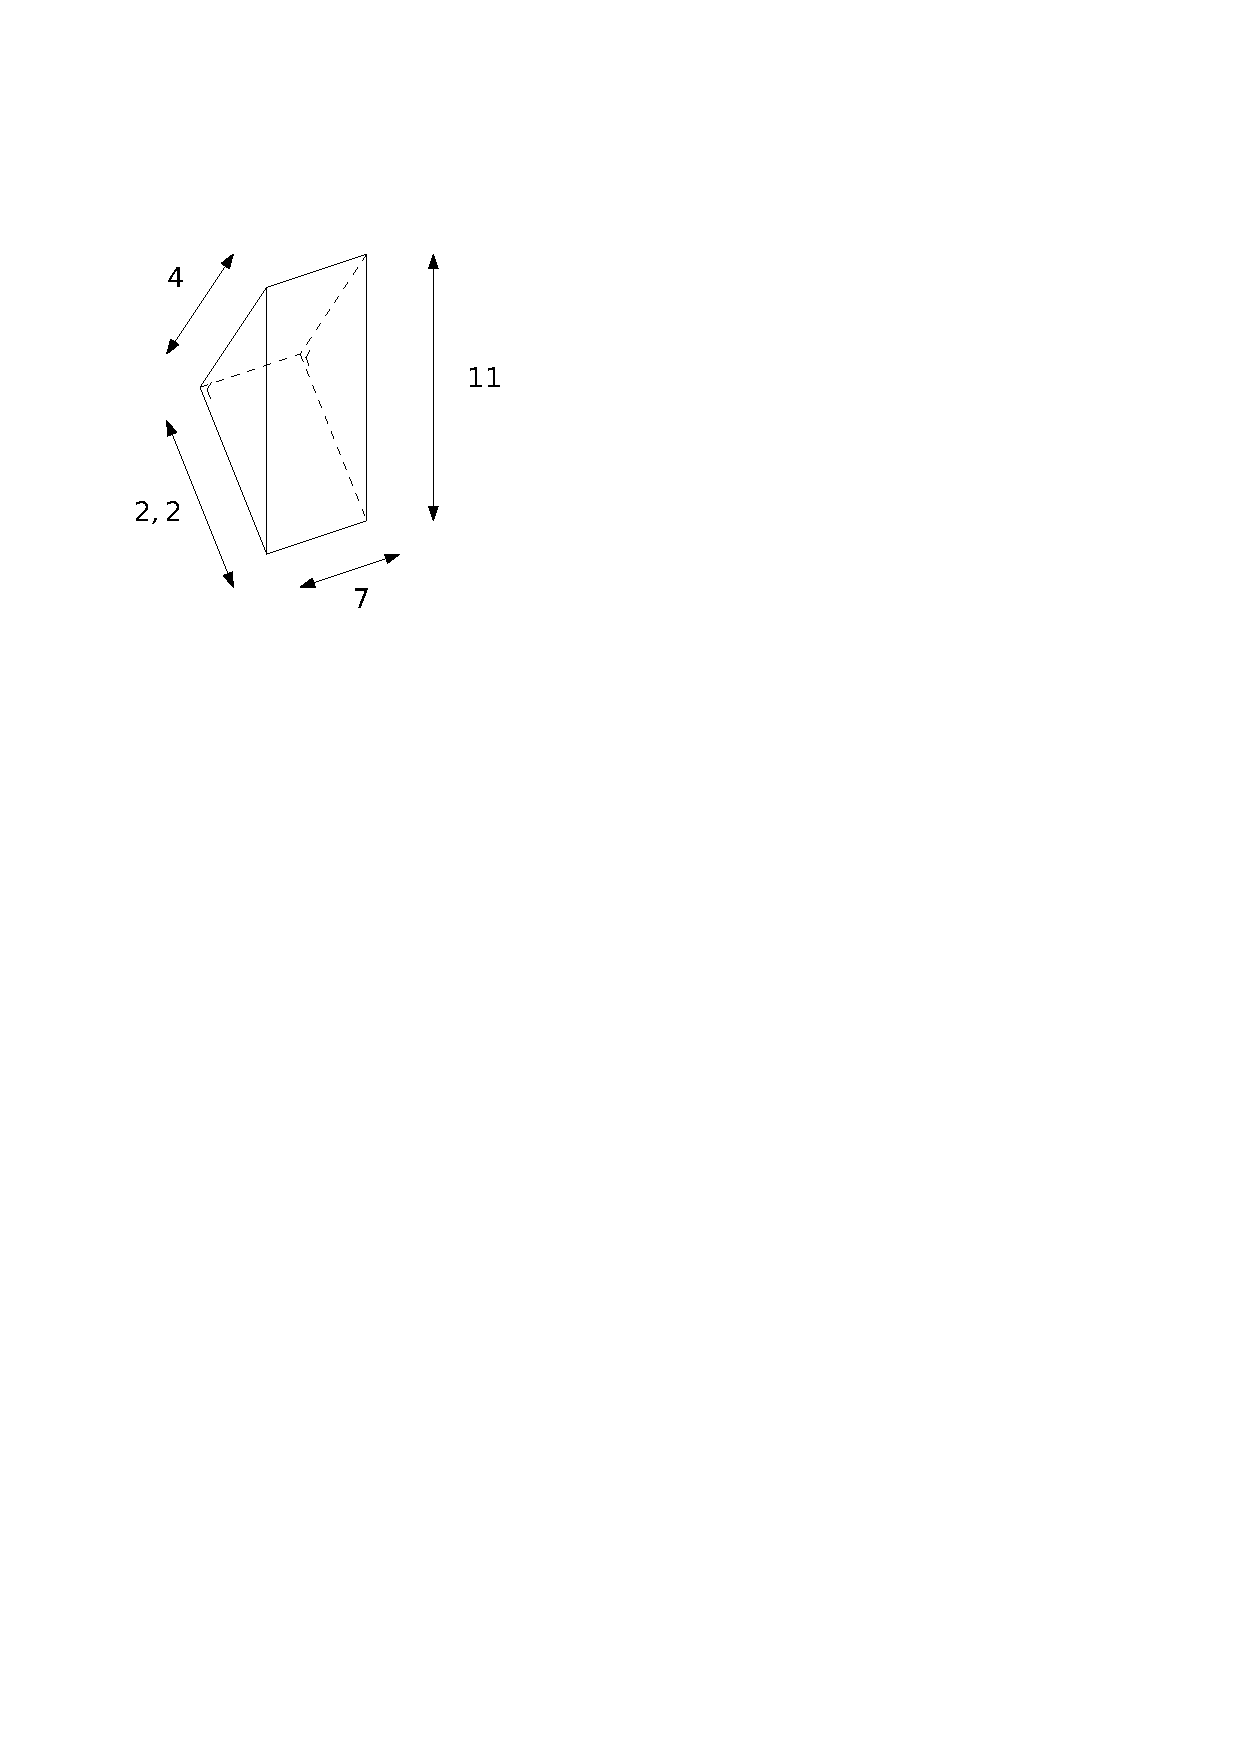
\includegraphics[scale=0.5]{media/gm-02/prisme-triang3.pdf}
    \task ~\\ 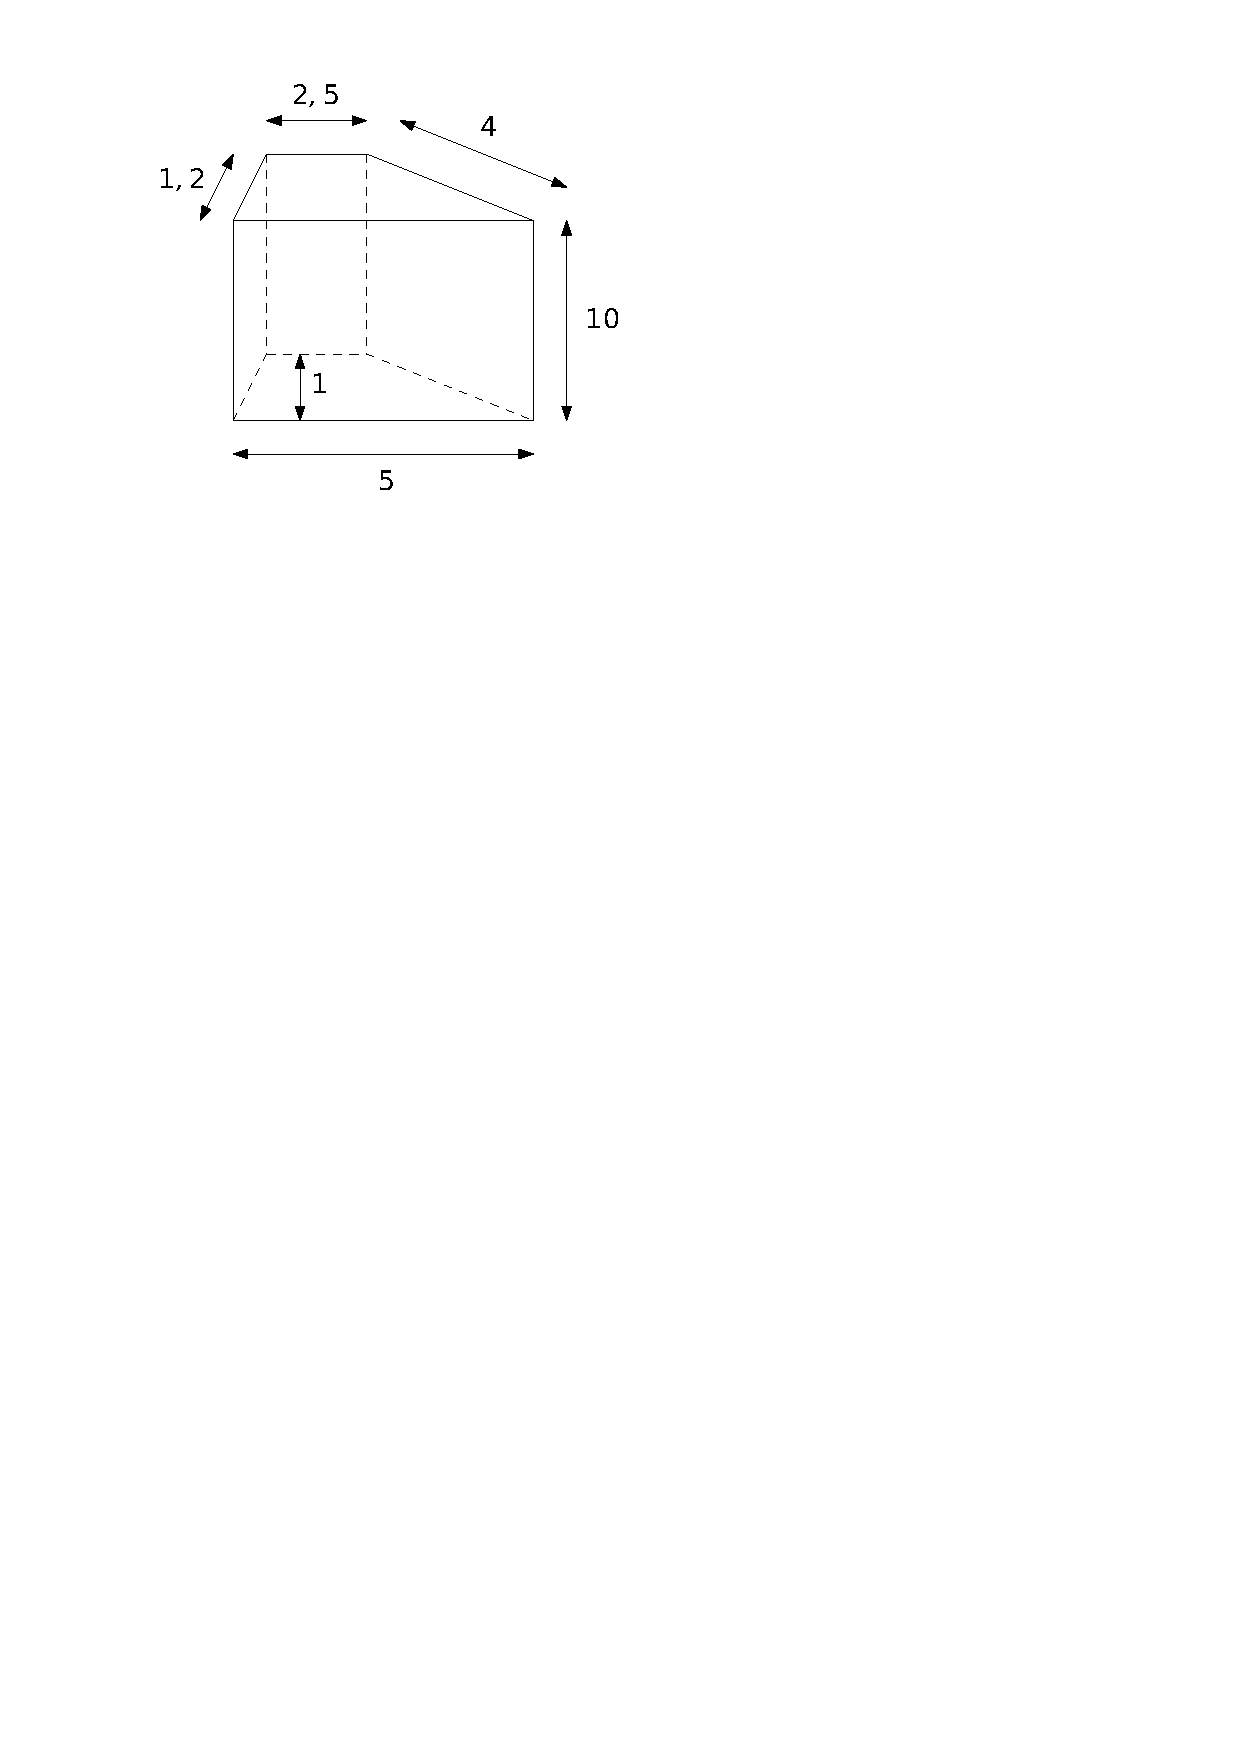
\includegraphics[scale=0.5]{media/gm-02/prisme-trap.pdf}
\end{tasks}
}{2}    
\end{exop}






\begin{QSJ}{197}{1}
\end{QSJ}

\end{document}$
